\documentclass[11pt,a4paper]{article}
\usepackage[utf8]{inputenc}
\usepackage{amsmath,amsfonts,amssymb,amsthm,epsfig,epstopdf,titling,url,array}
\usepackage{geometry}
\usepackage{algpseudocode}
\usepackage{algorithm}

%\usepackage{pgfplots}
\usepackage[all]{xy}
\usepackage{tikz}


\usepackage{biblatex}
\usepackage[title]{appendix}

\DeclareMathOperator{\Ima}{Im}


\newtheorem{theorem}{Theorem}
\newtheorem{procedure}{Procedure}
\newtheorem{lemma}{Lemma}
\newtheorem{definition}{Definition}
\newtheorem{example}{Example}




\begin{document}

\begin{center}
	\vspace*{1cm}
	
	\textbf{\Large Linear Impulsive Systems: Lie-Algebraic Techniques and Computational Tools}


	\vspace*{2cm}
	
	\text{A research project to the faculty of the School of Electrical Engineering and Computer Science}\\
	\text{Russ College of Engineering and Technology, Ohio University}\\
	\vspace*{0.4cm}
	\text{In partial fulfillment of the requirements for the degree of Master of Science}
	
	\vspace*{10cm}
	
	\textbf{Nghi M. V. Nguyen}\\
	August 15, 2018
	
	\vfill
	
	\vspace*{1cm}
\end{center}	

\pagebreak

\tableofcontents

\newpage

\listoffigures

\newpage

\section*{Abstract}
\qquad This research project will study the uniform exponential stability (UES) analysis for a class of linear impulsive systems using Lie algebraic techniques. The goal of the project is the computation of a Levi decomposition of the impulsive Lie algebra in which computational tools will be developed in a particular manner such that all algorithms must preserve nice numbers-integers or rational numbers and better illustrate the underlying theory and algorithms. The traditional MATLAB commands do not meet this objective. Computational tools will be designed to satisfy this aim. 

\section{Introduction}
\qquad An important class of hybrid systems is impulsive systems that consist of a mixture of continuous-time differential equations and discrete-time difference equations. In impulsive systems the continuous-time state variables undergo instantaneous changes or jumps caused by the nature of the systems or by the impulsive control laws (digital controllers). This phenomenon is of interest to scientists and engineers in a variety of applications. Of particular interests are sampled-data control systems and communication networks.

In this research project we investigate the uniform exponential stability (UES) analysis for a class of linear impulsive systems using Lie algebraic techniques. UES involves an exponentially decaying norm bound on the state trajectories that is uniform with respect to the initial time and sequence of impulse times. In [1] the author has successfully established the impulsive Lie algebra which is associated with the linear impulsive system and theoretically obtained sufficient conditions for the UES. From this paper, the solvability of the impulsive Lie algebra implies the UES of the system. Solvability means that every member of the Lie algebra can be represented as an upper triangular matrix in a common basis. In the case that the impulsive Lie algebra is not solvable, the Levi decomposition is employed and analyzed in which if a Levi factor in the decomposition is compact, then the system is also UES. This research project is the follow-up of these sufficient conditions in [1] in which we concentrate on computational aspects of the Levi decomposition.

Our contribution of this research is the development of MATLAB-based computational tools for the construction of the Lie algebra and related objects that preserve "nice" numbers (e.g. integers or rational numbers) in order to support the development of tutorial examples that illustrate the underlying theory.

The organization of this research report is arranged as follows; Section 1.1 will introduce linear impulsive systems, and Section 1.2 is about quadratic Lyapunov functions. Chapter 2 will provide essential mathematical background. The main part of the project will be described in Chapter 3. Chapter 4 presents an application of these tools to linear impulsive systems. Finally, Chapter 5 is the conclusion.

% 
\subsection{Linear Impulsive Systems}
	\qquad In this research work we investigate the uniform exponential stability analysis, using Lie-algebraic techniques, for the following class of linear impulsive systems
\begin{align*}
\dot{x}(t) &= \mathrm{A}_\mathcal{C}x(t) + \mathrm{B}_\mathcal{C}u(t) \quad t \notin \mathcal{T} \\
x(\tau_k) &= \mathrm{A}_\mathcal{I}x(\tau_k^{-}) + \mathrm{B}_\mathcal{I}u[k] \quad \tau_k \in \mathcal{T}, \text{ } k \in \mathbb{Z} \\
y(t) &= \mathrm{C}_\mathcal{C}x(t) + \mathrm{D}_\mathcal{C}u(t)  \\
y[k] &= \mathrm{C}_\mathcal{I}x(\tau^{-}_k) + \mathrm{D}_\mathcal{I}u[k]
\end{align*}
in which $x(t)$ is a continuous time state governed by the differential equation that undergoes jumps (instantaneous changes) at discrete times which are assumed to be a strictly increasing sequence in the set $\mathcal{T}$. Also, $u(t)$ and $u[k]$ are continuous-time and discrete-time control inputs, respectively, and $y(t)$ and $y[k]$ are continuous-time and discrete-time outputs, respectively. The matrices $\mathrm{A}_\mathcal{C}$, $\mathrm{B}_\mathcal{C}$, $\mathrm{C}_\mathcal{C}$, and $\mathrm{D}_\mathcal{C}$ are system data that describe the continuous-time dynamics whereas the matrices $\mathrm{A}_\mathcal{I}$, $\mathrm{B}_\mathcal{I}$, $\mathrm{C}_\mathcal{I}$, and $\mathrm{D}_\mathcal{I}$ are used to specify the discrete-time dynamics.\\
 
We restrict our stability analysis to a class of homogeneous linear impulsive systems with respect to an arbitrary sequence of impulse times. Specifically, we consider the linear impulsive system as described below
\begin{align}
\dot{x}(t) &= \mathrm{A}_\mathcal{C}x(t) \qquad t \notin \mathcal{T} \\
 x(\tau_k) &= \mathrm{A}_\mathcal{I}x(\tau_k^{-}) \qquad \tau_k \in \mathcal{T} \nonumber
\end{align}
where $\mathcal{T}$ is an arbitrary sequence of strictly increasing impulse times.\\

The sate transition matrix for the linear impulsive system (1) is given by $\Phi(t_f, t_0) = e^{\mathrm{A}_\mathcal{C}[t_f-t_0]}$ when $\mathcal{T}\cap(t_0,t_f] = \emptyset $ (no impulse effects from $t_0$ to $t_f$). Otherwise,
$$
\Phi(t_f, t_0) = e^{\mathrm{A}_\mathcal{C}[t_f-\tau_{\kappa(t_f)}]}\mathrm{A}_\mathcal{I}
\left( \prod^{\kappa(t_f)-1}_{j=\kappa(t_0)+1}e^{\mathrm{A}_\mathcal{C}[\tau_{j+1}-\tau_j]}\mathrm{A}_\mathcal{I} \right)
e^{\mathrm{A}_\mathcal{C}[\tau_{\kappa(t_0)+1}-t_0]}
$$
where the function $\kappa$ is a subsequent bookkeeping function from $\mathbb{R}$ to $\mathbb{Z}$ defined as
$$
\kappa(t) = \mathrm{sup}\{k \in \mathbb{Z} \text{ } \lvert \text{ } \tau_k \in \mathcal{T} \text{ and } \tau_k \leq t \}
$$

\textbf{Definition 1. Uniform Exponential Stability (UES)}. (see [2])
The system (1) is said to be uniformly exponentially stable if there exist positive constants $k$, $\lambda$ such that the state response satisfies
$$
\Vert x(t) \Vert \leq ke^{-\lambda(t-t_0)}\Vert x(t_0) \Vert, \quad \forall t \geq t_0
$$
for all initial times $t_0$, all initial states $x(t_0)$, and all impulse time sets $\mathcal{T}$.\\

\textbf{Example 1.} (From [1]) Let us consider a two-dimensional impulsive system (1) with data given by 
	$$
	\mathrm{A}_{\mathcal{C}} = 
	\begin{bmatrix}
 		-\mu & -\omega/ \rho \\
 		\omega \rho & -\mu
 	\end{bmatrix},  \qquad
	\mathrm{A}_{\mathcal{I}} = 
	\begin{bmatrix}
 		0 & -1 \\
 		1 & 0
 	\end{bmatrix}
 	$$
where $\mu$, $\omega$, and $\rho$ are positive. 
The continuous-time dynamics are exponentially stable and the impulsive dynamics produce an instantaneous 90-degree counterclockwise rotation of the state trajectory at the impulse times.\\

We demonstrate that for the case $\rho \neq 1$ there exist values of $\mu$ and $\omega$ for which the impulsive
system is not uniformly exponentially stable.  Specifically, there exists an initial state and a sequence of impulse times
that produce an unbounded state trajectory.
Without loss of generality, we assume $\rho > 1$; the case $\rho < 1$ can be addressed in a similar way.

Let us first analyze the continuous-time dynamics.  The eigenvalues of $A_\mathcal{C}$ are $- \mu \pm j \omega$,
thus the continuous-time dynamics produce a state trajectory that spirals to the origin for any initial state.
Specifically, for the initial state $x_0 = [ \begin{array}{cc} 1 & 0 \end{array} ]^T$, the state trajectory is given by
\begin{equation*}
\left[ \begin{array}{c} x_1 (t) \\ x_2 (t) \end{array} \right] =
e^{-\mu t} \left[ \begin{array}{c} \cos (\omega t) \\ \rho \sin (\omega t) \end{array} \right] , \quad t \ge 0
\end{equation*}
which consists of two parts.  The first part is the exponentially decaying factor $e^{-\mu t} $.  The second part
defines a periodic trajectory with period $T =  2 \pi / \omega$ that rotates in the counterclockwise direction along
the ellipse
\begin{equation*}
x_1^2 + \left( \frac{x_2}{\rho} \right)^2 = 1
\end{equation*}
For $\rho > 1$, the major axis of the ellipse lies along the $x_2-$axis and the minor axis of the ellipse lies along the $x_1-$axis.
As the elliptical portion of the trajectory transitions from the minor axis to the major axis over a quarter of the period,
its norm is expanded by the factor $\rho$.
Specifically, the norm of the given initial state equals 1 and the norm of
\begin{equation*}
\left[ \begin{array}{c} \cos (\omega T/4 ) \\ \rho \sin (\omega T/4) \end{array} \right]
=
\left[ \begin{array}{c} \cos (\pi /2 ) \\ \rho \sin (\pi /2) \end{array} \right]
=
\left[ \begin{array}{c} 0\\ \rho \end{array} \right]
\end{equation*}
is equal to $\rho$.
Over the next quarter period, the state transitions to
\begin{equation*}
\left[ \begin{array}{c} \cos (\omega T/2 ) \\ \rho \sin (\omega T/2) \end{array} \right]
=
\left[ \begin{array}{c} \cos (\pi ) \\ \rho \sin (\pi) \end{array} \right]
=
\left[ \begin{array}{c} -1 \\ 0 \end{array} \right]
\end{equation*}
whose norm once again equals 1.
This process repeats. The expansion of the elliptical trajectory as it transitions from minor axis to major axis over a quarter of a period
is immediately followed by a contraction over the next quarter of a period.\\

Even with the exponentially decaying factor, the norm of the continuous-time trajectory may still expand as it transitions minor axis to major axis.
This occurs when expansion by the factor $\rho > 1$ over a quarter of a period overcomes the exponential decay over that interval, that is, when
$\rho e^{-\mu T/4} = \rho e^{-\mu \pi / (2 \omega)} > 1$ or $\mu < \frac{2 \omega}{\pi} \ln \rho$.
When this is immediately followed by the ensuing contraction over the next quarter of a period along with the same exponential decay, the net effect over
half a period is a decay in norm by the factor $e^{-\mu T/2} = e^{-\mu \pi / \omega}$.
Ultimately, the continuous-time trajectory is norm bounded by $\rho e^{-\mu t}$ for all $t \ge 0$ and the trajectory spirals to the origin.
This is depicted in Figure 1 for the parameter values
\begin{equation*}
\rho = 3, \quad \mu = 0.25, \quad \omega =1
\end{equation*}
for which $\frac{2 \omega}{\pi} \ln \rho = 0.2581 > \mu$.\\

The continuous-time behavior described above for $\mu < \frac{2 \omega}{\pi} \ln \rho$ leads to an instability for the impulsive system when the
impulsive effects are timed to occur when the trajectory reaches the $x_2-$axis.
In this situation, the net expansion as the trajectory transitions from the $x_1$-axis to the $x_2-$axis according to the continuous-time dynamics
is immediately followed by an instantaneous norm-preserving
rotation back to the $x_1-$axis produced by the impulsive dynamics, thus bypassing the contraction phase of the continuous-time dynamics.
This results in an uninterrupted sequence of expansions yielding an unbounded trajectory for the impulsive system.\\

We conclude that for $\rho > 1$ and $\mu$, $\omega$ satisfying $\mu < \frac{2 \omega}{\pi} \ln \rho$, the impulsive system fails to be uniformly exponentially stable.
Simulations illustrate this phenomenon for the values of $\rho$, $\mu$, and $\omega $ given above.
For the same initial state $x(0) = x_0 = [ \begin{array}{cc} 1 & 0 \end{array} ]^T$
and the impulse time set
\begin{equation*}
\mathcal{T} = \{ \tau_k = k T/4 = k \pi/2 , \text{ } k = 1,...,10 \}
\end{equation*}
the phase portrait of the impulsive system is shown in Figure 2.
The individual state variable responses are plotted in Figures 3 and 4.
These responses depict an unbounded trajectory for the impulsive system for the specified
parameter values, initial state, and impulse time set.\\

Furthermore, when $\rho = 1$, the impulsive system is uniformly exponentially stable for any $\mu > 0$ and $\omega > 0$ (for any initial state and any sequence of impulse times). Indeed, this is a special case of the case $\rho \neq 1$ in which there is no expansion factor. The amount $e^{-\mu t}$ of the exponentially decaying factor is always less than one for any $\mu > 0$ and $\omega > 0$, and for all $t \geq 0$. Also, the impulse effects do not change the contraction phase of the trajectories.  Thus, from the analysis above for $\rho \neq 1$, the trajectories of the impulsive system spiral towards the origin without any expansion.\\
\\
\\

\begin{figure}
\centering
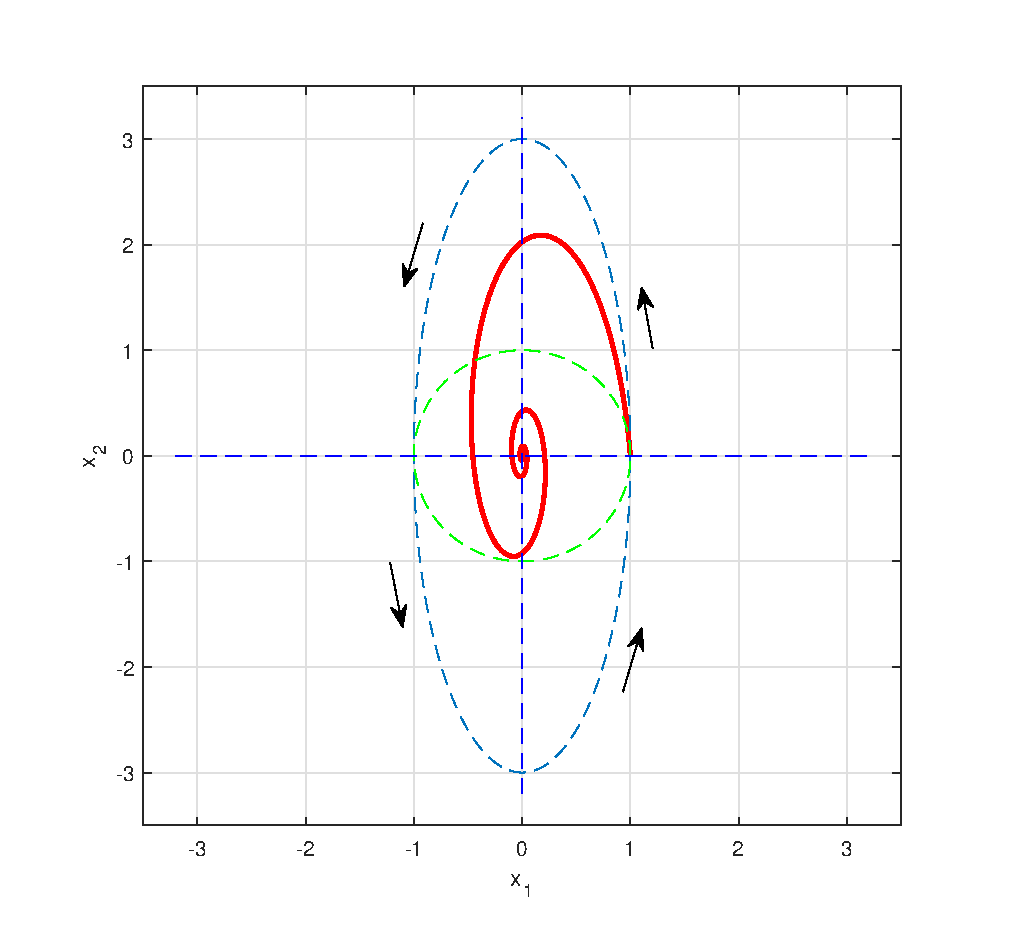
\includegraphics[scale=0.6]{FG1A.eps} 
\caption{Phase Portrait without impulse effects}
\end{figure}

\begin{figure}
\centering
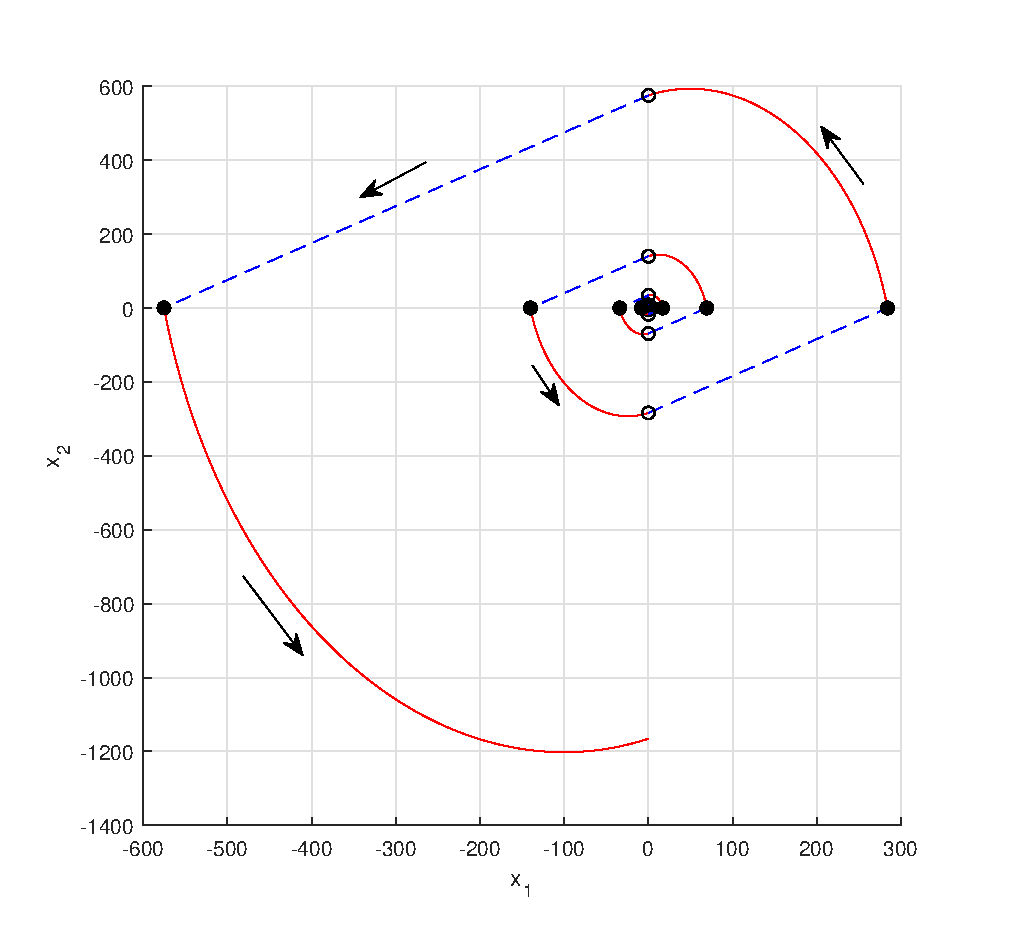
\includegraphics[scale=0.6]{FG2.eps} 
\caption{Phase Portrait with impulse effects}
\end{figure}

\begin{figure}
\centering
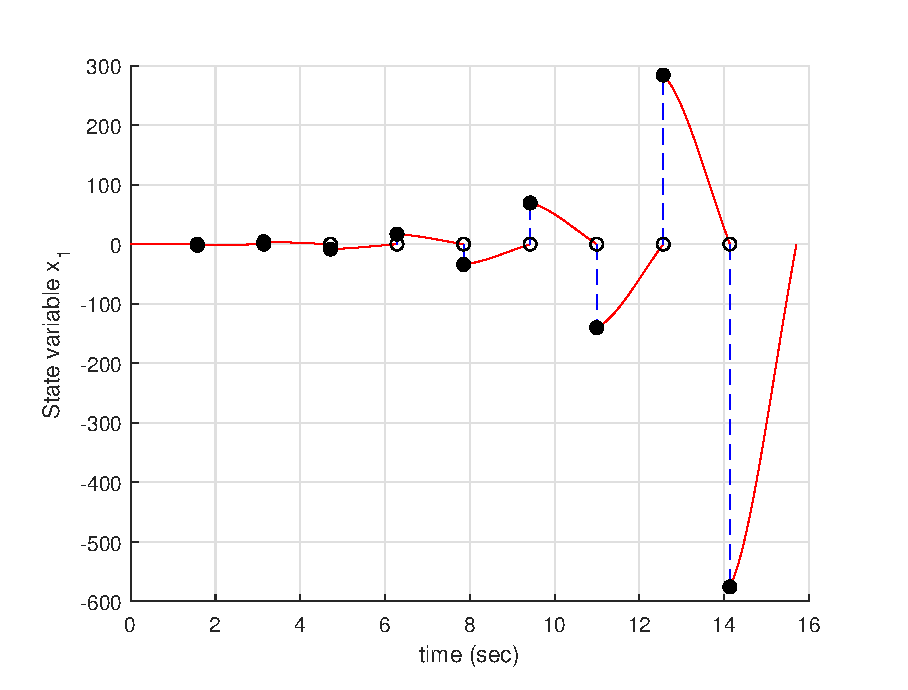
\includegraphics[scale=0.8]{FG3.eps} 
\caption{Initial Value Response $x_1(t)$ vs $t$}
\end{figure}

\begin{figure}
\centering
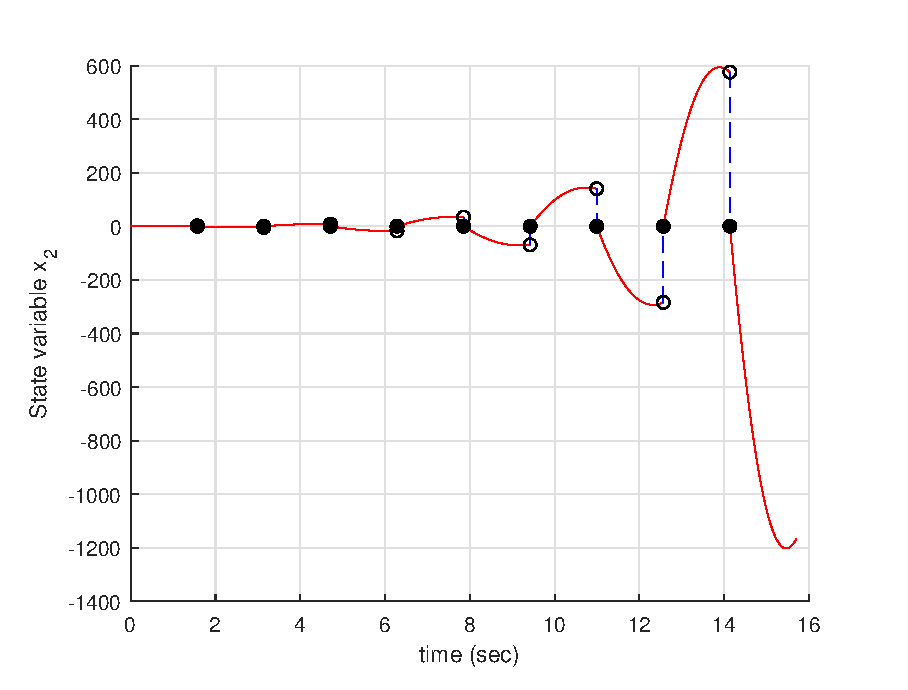
\includegraphics[scale=0.8]{FG4.eps} 
\caption{Initial Value Response $x_2(t)$ vs $t$}
\end{figure}


%
\subsection{Quadratic Lyapunov Functions}
	\quad \text{ } \textbf{Definition 2.} A symmetric matrix $P$ is called a positive definite (semidefinite) matrix if all of its leading principal minors are positive (nonnegative). Equivalently, all eigenvalues of $P$ are positive (nonnegative), or
$x^TPx > 0$ ($x^TPx \geq 0$), $0 \neq x \in \mathbb{R}^n$. If
$-x^TPx > 0$ ($-x^TPx \geq 0$), $0 \neq x \in \mathbb{R}^n$, $P$
is called  negative definite (semidefinite).\\
	
	\textbf{Example 2.}
	$P =
	\begin{bmatrix}
 		 1 & -1 & -1 \\
 		-1 &  5 &  1 \\
 		-1 &  1 &  5
 	\end{bmatrix}$
is symmetric positive definite as verified bellow
$$
p_{11} = 1 > 0, \quad
p_{22}= \mathrm{det}
\begin{bmatrix}
 		 1 & -1 \\
 		-1 &  5
 	\end{bmatrix}
 	= 4 > 0, \quad
p_{33} = \mathrm{det}
	\begin{bmatrix}
 		 1 & -1 & -1 \\
 		-1 &  5 &  1 \\
 		-1 &  1 &  5
 	\end{bmatrix}
 	= 16 > 0.
$$

\textbf{Definition 3.} For the continuous-time system $\dot{x}(t) = \mathrm{A}x(t)$,
the function $V(x) = x^TPx$ is a quadratic Lyapunov function (QLF) for the system if $P$ is symmetric positive definite and $\mathrm{A}^TP + P\mathrm{A} \leq 0$ (negative semidefinite).\\

\textbf{Definition 4.} The derivative of $V(x) = x^TPx$ along the trajectories of the continuous dynamics is defined by
$$
\dot{V}(x) = \frac{\partial V}{\partial x}(x)\mathrm{A}(x) = x^T[\mathrm{A}^TP + P\mathrm{A}]x
$$
$\dot{V}(x)$ is also a quadratic form expressed in terms of the symmetric matrix $\mathrm{A}^TP + P\mathrm{A}$.\\

\textbf{Definition 5.} For the discrete-time system $x[k+1] = \mathrm{A}x[k]$,
the function $V(x) = x^TPx$ is a quadratic Lyapunov function (QLF) for the system if $Q$ is symmetric positive definite and $\mathrm{A}^TP\mathrm{A} - P \leq 0$.\\

\textbf{Definition 6.} The difference of $V(x) = x^TPx$ along the trajectories of the discrete-time system
$x[k+1] = \mathrm{A}x[k]$ is defined by
$$
\Delta V(x) = x^T[\mathrm{A}^TP\mathrm{A} - P]x
$$
 
The system (1) can be viewed as a mixed combination of continuous and discrete dynamics. Hence, it is natural to establish a Lyapunov-type criterion for the uniform exponential stability of (1). Precisely, the result is presented in the following theorem.
	
\begin{theorem}(see [2]) If there exists a common symmetric positive definite matrix $P$ that satisfies the inequalities 
	\begin{align}
	\mathrm{A}^T_{\mathcal{C}}P + P\mathrm{A}_{\mathcal{C}} &< 0  \\
	\mathrm{A}^T_{\mathcal{I}}P\mathrm{A}_{\mathcal{I}} - P &< 0 \nonumber
	\end{align}
	Then, the system (1) is uniformly exponentially stable. Let $V(x)= x^TPx$. Its derivative along the trajectories satisfies
	$$\dot{V}[x(t)] < 0, \text{ } t \in [\tau_k, \tau_{k+1}), \quad  V[x(\tau_k)]- V[x(\tau_k^-)] < 0, \quad \forall \text{ } t_0, \text{ } \forall \text{ }\mathcal{T}. $$
	 Thus, $V(x)$ can be thought of as a common quadratic Lyapunov function for (1).\\
\end{theorem}

%
%
\section{Mathematical Background}
\qquad In this section we will present fundamental concepts and important results in Lie algebra theory that relate to the study of uniform exponential stability of linear impulsive systems.
\subsection{Matrix Lie Algebras}
\quad \textbf{ Definition 7.} Let $\mathbb{F}$ be a field ($\mathbb{C}$ or $\mathbb{R}$). An $\mathbb{F}$-vector space $\mathsf{L}$ along with a bilinear function $[\cdot,\cdot]$, the Lie bracket, is called a Lie algebra if ($\mathsf{L}$, $[\cdot,\cdot]$) satisfies the following postulates 
\begin{align*}
&[X,X] = 0 \quad \forall X \in \mathsf{L}, \\
&[X,[Y,Z]]+[Y,[Z,X]]+[Z,[X,Y]] = 0 \quad \forall X,Y,Z \in \mathsf{L}.
\end{align*}

\textbf{Example 3.} Let us consider the vector space of all $n \times n$ matrices over $\mathbb{C}$, denoted by $\mathfrak{gl}(n,\mathbb{C})$, with the Lie bracket defined by
$$
[X,Y] = XY - YX
$$
in which $XY$ is the normal product of the two matrices $X$ and $Y$. It is not difficult to check this Lie bracket satisfies the two postulates in Definition 6. Thus, $\mathfrak{gl}(n,\mathbb{C})$ is a Lie algebra.\\

\textbf{Definition 8.} The Lie algebra $\mathfrak{gl}(n,\mathbb{C})$ is called the general linear algebra.
\\

\textbf{Definition 9.} Let $X$ be a fixed element of a Lie algebra $\mathsf{L}$. The adjoint operator $\mathrm{ad}_X$ is a linear operator from $\mathsf{L}$ into $\mathsf{L}$ defined by
\begin{center}
$\mathrm{ad}_X: \mathsf{L} \longrightarrow \mathsf{L}$ \\
$\mathrm{ad}_X Y = [X,Y]$
\end{center}

\textbf{Definition 10.} Let $\mathsf{L}$ be a Lie algebra. A Lie subalgebra $\mathsf{S}$ of $\mathsf{L}$ is a vector subspace of $\mathsf{L}$ that is closed under the Lie bracket, i.e.,
$$
[X,Y] \in \mathsf{S}, \quad \forall X, Y \in \mathsf{S}.
$$ 
A Lie subalgebra of the general linear algebra $\mathfrak{gl}(n,\mathbb{C})$ is called a matrix Lie algebra.\\

\textbf{Example 4.} (see [9]) The subspace of all upper triangular matrices, $\mathsf{b}(n,\mathbb{C})$, and the subspace of all strictly upper triangular matrices, $\mathsf{n}(n,\mathbb{C})$, of $\mathfrak{gl}(n,\mathbb{C})$ are matrix Lie algebras.\\

\textbf{Example 5.} The special Lie algebra $\mathfrak{sl}(n,\mathbb{C})$, defined by
$$
\mathfrak{sl}(n,\mathbb{C}) = \{ X \in \mathfrak{gl}(n,\mathbb{C}) \text{ }\vert \text{ } \mathsf{tr}(X) = 0 \}
$$
is also a Lie subalgebra of $\mathfrak{gl}(n,\mathbb{C})$  and so is a matrix Lie algebra.\\

\textbf{Definition 11.} An ideal $\mathsf{I}$ of a Lie algebra $\mathsf{L}$ is a subspace of $\mathsf{L}$ such that $[\mathsf{L},\mathsf{I}] \subset \mathsf{I}$. Obviously, $\mathsf{I}$ is also a Lie subalgebra of $\mathsf{L}$.\\

\textbf{Example 6.} The special Lie algebra $\mathfrak{sl}(n,\mathbb{C})$ is an ideal of $\mathfrak{gl}(n,\mathbb{C})$. The Lie algebra
$\mathsf{n}(n,\mathbb{C})$ is an ideal of
$\mathsf{b}(n,\mathbb{C})$. But $\mathsf{b}(n,\mathbb{C})$ is not an ideal of $\mathfrak{gl}(n,\mathbb{C})$.\\

Let $\mathsf{L}$ be a $d$-dimensional Lie algebra and let $\mathfrak{B} = \{X_1, X_2, \dots, X_d \}$ denote a basis for $\mathsf{L}$ (as a vector space). It is possible to express Lie brackets of each pair of basis vectors (elements of $\mathfrak{B}$) as linear combinations of themselves. In other words, there exist scalars $c^i_{k,j}$ for which
$$
[X_k, X_j] = \sum _{i=1}^d c^i_{k,j} X_i, \quad 1 \leq k,j \leq d
$$

\textbf{Definition 12.} The scalars $c^i_{k,j}$ in the expression above are called the structure constants of $\mathsf{L}$. The number of structure constants is $d^3$. Also, the structure constants do depend on the basis of $\mathsf{L}$.\\

For any fixed $k$, $1 \leq k \leq d$, let us rewrite the expression above in operator form as
$$
\mathrm{ad}_{X_k} X_j = \sum _{i=1}^d c^i_{k,j} X_i, \quad 1 \leq j \leq d
$$
This defines a matrix representation for the adjoint operator $\mathrm{ad}_{X_k}$ as below.\\

\textbf{Definition 13.} A matrix representation of $\mathrm{ad}_{X_k}$ is
$
[\mathrm{ad}_{X_k}] = [c^i_{k,j}]
$
in which $i$ is the row index and $j$ is the column index.\\

\textbf{Definition 14.} (see [9]) The Killing form on a Lie algebra $\mathsf{L}$ is the symmetric bilinear form $\mathcal{K}: \mathsf{L} \times \mathsf{L} \rightarrow \mathbb{F}$ defined by
$$
\mathcal{K}(X,Y) = \mathsf{tr}(\mathrm{ad}_X \circ \mathrm{ad}_Y), \text{ } X, Y \in \mathsf{L}
$$
in which $\mathrm{ad}_X$ and $\mathrm{ad}_Y$ denote the adjoint operators with respect to $X$ and $Y$, respectively. Also, the Killing form satisfies the invariance property
$$
\mathcal{K}(X,[Y,Z]) = \mathcal{K}([X,Y],Z), \text{ }
X,Y,Z \in \mathsf{L}
$$

\textbf{Example 7.}(From [12]) Let $\mathsf{L}$ be a 2-dimensional Lie algebra with a basis  $\{ X_1, X_2 \}$. Define the Lie bracket on the basis as 
$$[X_1, X_2] = X_1$$
Recall that $[X_1, X_1] = 0$ and $ [X_2, X_2] = 0$. To find the Killing form on $\mathsf{L}$, we first calculate adjoint operators with respect to $X_1$ and $X_2$. From Definition 9, we have
$$
\mathrm{ad}_{X_1}X_1 = [X_1, X_1] \text{ } = \text{ } 0, \quad
\mathrm{ad}_{X_1}X_2 = [X_1, X_2] = X_1
$$
$$ 
\mathrm{ad}_{X_2}X_1 = [X_2, X_1] = -X_1, \quad
\mathrm{ad}_{X_2}X_2 = [X_2, X_2] = 0
$$
Thus, the matrix representations for $\mathrm{ad}_{X_1}$ and $\mathrm{ad}_{X_2}$ with respect to the given basis are
$$
[\mathrm{ad}_{X_1}] = 
	\begin{bmatrix}
 		0 & 1 \\
 		0 & 0
 	\end{bmatrix}
 	, \quad
[\mathrm{ad}_{X_2}] = 
	\begin{bmatrix}
 		-1 & 0 \\
 		0 & 0
 	\end{bmatrix}
$$
We now compute the Killing form
\begin{align*}
\mathcal{K}(X_1,X_1) &= \mathrm{tr}(\mathrm{ad}_{X_1} \circ \mathrm{ad}_{X_1}) = 0 \\
\mathcal{K}(X_1,X_2) &= \mathrm{tr}(\mathrm{ad}_{X_1} \circ \mathrm{ad}_{X_2}) = 0 \\
\mathcal{K}(X_2,X_1) &= \mathrm{tr}(\mathrm{ad}_{X_2} \circ \mathrm{ad}_{X_1}) = 0 \\
\mathcal{K}(X_2,X_2) &= \mathrm{tr}(\mathrm{ad}_{X_2} \circ \mathrm{ad}_{X_2}) = 1
\end{align*}
The matrix representation for $\mathcal{K}$ is  
$
[\mathcal{K}] = 
	\begin{bmatrix}
 		0 & 0 \\
 		0 & 1
 	\end{bmatrix}
$
which is positive semi-definite.\\
 	
Next, we introduce the concept of orthogonal subspaces of $\mathsf{L}$ with respect to the Killing form.\\

\textbf{Definition 15.} Let $\mathcal{K}$ be a Killing form on $\mathsf{L}$ and $\mathsf{S}$ be a subspace of $\mathsf{L}$. The orthogonal (perpendicular) subspace to $\mathsf{S}$ is defined by
$$
\mathsf{S}^{\perp} = \{ X \in \mathsf{L} \text{ } \lvert \text{ } \mathcal{K}(X,S) = 0, \text{ } \forall S \in \mathsf{S} \}
$$

We note that if $\mathsf{I}$ is an ideal of $\mathsf{L}$, then the orthogonal subspace $\mathsf{I}^{\perp}$ to $\mathsf{I}$ is also an ideal of $\mathsf{L}$ as a consequence of the invariance property of the Killing form (see [9]).

%
\subsection{Impulsive Lie Algebra}
\qquad We now briefly introduce the impulsive Lie algebra associated with the impulsive system (1). Let $\mathcal{X} = \mathbb{C}^n$ be the underlying vector space. The impulsive Lie algebra $\mathsf{L}$ for system (1)  is a Lie subalgebra of the general matrix algebra $\mathfrak{gl}(n,\mathbb{C})$ generated by the following set (see [1])
$$
\mathfrak{G}=\{\mathrm{A}_k = \mathrm{A}_\mathcal{I}^{-k}\mathrm{A}_\mathcal{C}\mathrm{A}_\mathcal{I}^k, \quad k \geq 0 \}
$$
in which $\mathrm{A}_\mathcal{C} \in \mathfrak{gl}(n,\mathbb{C})$, and $\mathrm{A}_{\mathcal{I}}$
is assumed to be invertible or $\mathrm{A}_{\mathcal{I}}\in \mathrm{GL}(n,\mathbb{C})$, the general linear group. Specifically, $\mathsf{L}$ is the $\mathbb{C}$-linear span of elements of $\mathfrak{G}$ of the form
$$
[\mathrm{A}_{k_r},[\mathrm{A}_{k_{l-1}},[..., [\mathrm{A}_{k_2},\mathrm{A}_{k_1}]...]]],
\text{  }\mathrm{A}_{k_j} \in \mathfrak{G},
\text{  } j = 1,...,r \text{ and } r>0.
$$

Geometrically, $\mathsf{L}$ can be characterized in terms of a subspace of $\mathfrak{gl}(n,\mathbb{C})$ that is invariant with respect to certain maps. For this purpose we employ the adjoint operator and the adjoint map that have this property. \\

\textbf{Definition 16.} Let $\mathrm{A} \in \mathfrak{gl}(n,\mathbb{C})$ and $\mathrm{g} \in \mathrm{GL}(n,\mathbb{C})$. The adjoint operator $\mathrm{ad}_{\mathrm{A}}$ and the adjoint map $\mathrm{Ad}_{\mathrm{g}}$ are defined respectively by  
$$
\mathrm{ad}_{\mathrm{A}}: \mathfrak{gl}(n,\mathbb{C}) \longrightarrow  \mathfrak{gl}(n,\mathbb{C})
$$
$$
\mathrm{ad}_{\mathrm{A}} X = [\mathrm{A},X]
$$
$$
\mathrm{Ad}_{\mathrm{g}}: \mathfrak{gl}(n,\mathbb{C}) \longrightarrow  \mathfrak{gl}(n,\mathbb{C})
$$
$$
\mathrm{Ad}_{\mathrm{g}} X = \mathrm{g}X\mathrm{g}^{-1}
$$

With respect to these two maps for
$\mathrm{A}_\mathcal{C} \in \mathfrak{gl}(n,\mathbb{C})$ and $\mathrm{A}_\mathcal{I} \in \mathrm{GL}(n,\mathbb{C})$,
$\mathsf{L}$ is the smallest $subspace$ of $\mathfrak{gl}(n,\mathbb{C})$ that is invariant under both $\mathrm{ad}_{\mathrm{A}_\mathcal{C}}$ and $\mathrm{Ad}_{\mathrm{A}_{\mathcal{I}}}$ and contains $\mathrm{span}\{\mathrm{A}_\mathcal{C}\}$. From [1], $\mathsf{L}$ can be recursively computed by the following algorithm
\begin{align*}
\mathsf{L}_0 &= \langle \mathrm{Ad}_{\mathrm{A}_{\mathcal{I}}} \text{ }| \text{ } \mathrm{span}\{\mathrm{A}_\mathcal{C}\} \rangle \\
\mathsf{L}_k &= \mathsf{L}_{k-1} + \langle \mathrm{Ad}_{\mathrm{A}_{\mathcal{I}}} \text{ }| \text{ } \mathrm{ad}_{\mathrm{A}_\mathcal{C}}\mathsf{L}_{k-1} \rangle \quad k \geq 1
\end{align*}
in which the notation $\langle \mathrm{Ad}_{\mathrm{A}_{\mathcal{I}}} \text{ }| \text{ } \mathrm{span}\{\mathrm{A}_\mathcal{C}\} \rangle$ means the minimal (smallest) subspace that is invariant under the map $\mathrm{Ad}_{\mathrm{A}_{\mathcal{I}}}$ and contains
$\mathrm{span}\{\mathrm{A}_\mathcal{C}\}$.

%
\subsection{Solvable, Nilpotent, and Abelian Lie Algebras}
\quad \textbf{ Definition 17.} Let $\mathsf{L}$ be a Lie algebra. The derived series of $\mathsf{L}$ is the series of terms
$$
\mathsf{L}^{(k)} = [\mathsf{L}^{(k-1)},\mathsf{L}^{(k-1)}], \quad k > 1.
$$
The derived series of $\mathsf{L}$ is a decreasing series of ideals, i.e., $\mathsf{L} \supset \mathsf{L}^{(1)} \supset \mathsf{L}^{(2)} \supset ... $\\

\textbf{Definition 18.} The Lie algebra $\mathsf{L}$ is said to be solvable if there exists an integer $r \geq 1$ such that $\mathsf{L}^{(r)} = 0$.\\

\textbf{Example 8.} The Lie algebra $\mathsf{L} = \mathsf{b}(n,\mathbb{C})$ of upper triangular matrices over $\mathbb{C}$ is a solvable algebra.\\

\textbf{Definition 19.} The lower central series of a Lie algebra $\mathsf{L}$ is the series of terms
\begin{align*}
\mathsf{L}^1   &= [\mathsf{L},\mathsf{L}] \\
\mathsf{L}^{k} &= [\mathsf{L},\mathsf{L}^{k-1}], \quad k > 1.
\end{align*}
The lower central series of $\mathsf{L}$ is also a decreasing series of ideals i.e., $\mathsf{L} \supset \mathsf{L}^{1} \supset \mathsf{L}^{2} \supset ... $\\

The first term in both the derived and lower central series
$\mathsf{L}^{(1)} = \mathsf{L}^1 = [\mathsf{L},\mathsf{L}]$
is called the derived algebra. \\

\textbf{Definition 20.} The Lie algebra $\mathsf{L}$ is said to be nilpotent if there exists an integer $r \geq 1$ such that $\mathsf{L}^{r} = 0$. If $\mathsf{L}$ is nilpotent then $\mathsf{L}$ is solvable.\\

\textbf{Example 9.} The Lie algebra $\mathsf{L} = \mathsf{n}(n,\mathbb{C})$ of strictly upper triangular matrices over $\mathbb{C}$ is a nilpotent algebra. Furthermore, if $n \geq 2$ then $\mathsf{b}(n,\mathbb{C})$ is solvable but not nilpotent.\\

\textbf{Definition 21.} A Lie algebra $\mathsf{L}$ is said to be Abelian or commutative if $[\mathsf{L},\mathsf{L}] = 0$. Obviously, if $\mathsf{L}$ is Abelian then $\mathsf{L}$ is nilpotent and solvable.
\\

\textbf{Definition 22.} Let $\mathsf{L}$ be a Lie algebra. The center of $\mathsf{L}$ is an ideal of $\mathsf{L}$ defined by 
$$ \mathcal{C}(\mathsf{L}) = \{ x \in \mathsf{L} \text{ } \vert \text{ } [x,\mathsf{L}] = 0 \} $$

\textbf{Example 10.} The center $\mathcal{C}(\mathsf{L})$ is an Abelian Lie algebra.\\
 
\textbf{Definition 23.} Let $\mathsf{L}$ be a Lie algebra. The radical of $\mathsf{L}$, denoted by $\mathsf{Rad}(\mathsf{L})$, is the maximal solvable ideal of $\mathsf{L}$, i.e. the unique solvable ideal that contains all other solvable ideals.\\

\textbf{Definition 24.} A Lie algebra $\mathsf{L}$ is said to be semisimple if it has no non-zero solvable ideal, i.e. its only solvable ideal is zero.\\

\textbf{Remark 1.} If the radical  of $\mathsf{L}$ is equal to $\mathsf{L}$, $\mathsf{L}$ is solvable, and if $\mathsf{Rad}(\mathsf{L})$ is zero, then  $\mathsf{L}$ is semisimple.\\

\textbf{Remark 2.} The Killing form of a semisimple  Lie algebra $\mathsf{L}$ is nondegenerate, i.e.  $\mathcal{K} (X, X) \neq 0$ for all nonzero $X \in \mathsf{L}$.\\

\textbf{Definition 25.} A semisimple  Lie algebra $\mathsf{L}$ is compact if its Killing form is negative definite, i.e. $\mathcal{K} (X, X) < 0$ for all nonzero $X \in \mathsf{L}$.\\

\textbf{Definition 26.} If the radical of a Lie algebra $\mathsf{L}$ is also its center, i.e. $\mathsf{Rad}(\mathsf{L})= \mathcal{C}(\mathsf{L})$, then $\mathsf{L}$ is said to be reductive.\\

The following theorem actually provides an algorithm for computing the radical.

\begin{theorem}(see [7,8]) The radical of a Lie algebra $\mathsf{L}$ can be characterized through the Killing form as
\begin{align*}
\mathsf{Rad}(\mathsf{L}) & = \{ X \in \mathsf{L} \text{ } \lvert \text{ } \mathcal{K}(X,Y) = 0, \text{ } \forall  \text{ } Y \in [\mathsf{L},\mathsf{L}]  \} = [\mathsf{L},\mathsf{L}]^{\perp}
\end{align*}
\end{theorem}

%
\subsection{Levi Decomposition}
\qquad The structure of solvable Lie algebras is somewhat simple (similar to simultaneously upper triangular matrices) but not every Lie algebra is solvable in general. Fortunately, for any Lie algebra $\mathsf{L}$, there exists a semisimple subalgebra $\mathsf{S}$ of $\mathsf{L}$ such that $\mathsf{L}$ can be decomposed as a direct sum of its radical and $\mathsf{S}$. This is the content of Levi's Theorem.

\begin{theorem}(\textbf{Levi's Theorem})(see [7,10]) For any Lie algebra $\mathsf{L}$, there exists a semisimple subalgebra $\mathsf{S}$ of $\mathsf{L}$ such that
$\mathsf{L} = \mathsf{Rad}(\mathsf{L}) \oplus \mathsf{S}$.
$\mathsf{S}$ is called a Levi factor or a Levi subalgebra of $\mathsf{L}$.
\end{theorem}

The remainder of this document will present algorithms and related knowledge for computing a Levi decomposition of the impulsive Lie algebra $\mathsf{L}$ in the reductive case.

%
%
\section{Algorithms}
\qquad This section includes the main content of the document. We first introduce Kronecker product of two matrices. Then matrix representations for $\mathrm{ad}_{A}$ and $\mathrm{Ad}_{g}$ follow. In the last subsection a sequence of algorithms will be described in which the algorithm for computing a Levi factor is the last one.
\subsection{Kronecker Product}
	\qquad Let $\mathrm{A}$ be an $m_1$-by-$n_1$ matrix and $\mathbf{B}$ an $m_2$-by-$n_2$  (See [11]).
\begin{align*}
	\mathrm{A} = 
	\begin{bmatrix}
 		a_{11} & a_{12} & \ldots & a_{1n_1} \\
 		a_{21} & a_{22} & \ldots & a_{2n_1} \\
 		\vdots & \vdots & \ddots & \vdots \\
 		a_{m_1 1} & a_{m_1 2} & \ldots & a_{m_1 n_1} 
	\end{bmatrix},
	\quad
	\mathbf{B} = 
	\begin{bmatrix}
 		b_{11} & b_{12} & \ldots & b_{1n_2} \\
 		b_{21} & b_{22} & \ldots & b_{2n_2} \\
 		\vdots & \vdots & \ddots & \vdots \\
 		b_{m_2 1} & b_{m_2 2} & \ldots & b_{m_2 n_2} 
	\end{bmatrix}.
\end{align*}	
	The Kronecker product of $\mathrm{A}$ and $\mathbf{B}$ is an $m_1m_2$-by-$n_1n_2$ block matrix denoted by $\mathrm{A} \otimes \mathbf{B}$ and defined by
\begin{equation*}
\mathrm{A} \otimes \mathbf{B} =
\begin{bmatrix}
 a_{11}\mathbf{B} & a_{12}\mathbf{B} & \ldots & a_{1n_1}\mathbf{B} \\
 a_{21}\mathbf{B} & a_{22}\mathbf{B} & \ldots & a_{2n_1}\mathbf{B} \\
 \vdots & \vdots & \ddots & \vdots \\
 a_{m_11}\mathbf{B} & a_{m_12}\mathbf{B} & \ldots & a_{m_1n_1}\mathbf{B} 
\end{bmatrix}
\end{equation*}
Specifically, each block ($m_2$-by-$n_2$) of $\mathrm{A} \otimes \mathbf{B}$ is made up by multiplying $\mathbf{B}$ by each element of $\mathrm{A}$.\\

\textbf{Example 11.}
	$
	\mathrm{A} = 
	\begin{bmatrix}
 		1 & -1 \\
 		0 & 2
 	\end{bmatrix}
 	$,
 	$
	\mathrm{B} = 
	\begin{bmatrix}
 		2 & 0 \\
 		1 & -1
 	\end{bmatrix}.
 	$
 	The Kronecker product of $\mathrm{A}$ and $\mathrm{B}$ is\\
\\
$$
\mathrm{A} \otimes \mathrm{B} =
\left[
\begin{array}{c|c}
1\cdot \begin{bmatrix}
 		2 & 0 \\
 		1 & -1
 	\end{bmatrix} & -1\cdot \begin{bmatrix}
 		2 & 0 \\
 		1 & -1
 	\end{bmatrix} \\
\hline
0\cdot \begin{bmatrix}
 		2 & 0 \\
 		1 & -1
 	\end{bmatrix} & 2\cdot \begin{bmatrix}
 		2 & 0 \\
 		1 & -1
 	\end{bmatrix}
\end{array}
\right]
=
\begin{bmatrix}
 		2 &  0 & -2 & 0 \\
 		1 & -1 & -1 & 1 \\
 		0 &  0 &  4 & 0 \\
 		0 &  0 &  2 & -2
\end{bmatrix}
$$

%
\subsection{Matrix Representation for $\mathrm{ad}_{A}$ and $\mathrm{Ad}_{g}$}
\qquad  Let us consider the vector space of all $n\times n$ matrices over $\mathbb{C}$, $\mathfrak{gl}(n,\mathbb{C})$ or $\mathbb{C}^{n\times n}$ and the vector space of all $n^2\times 1$ vectors over $\mathbb{C}$, $\mathbb{C}^{n^2}$. If we rearrange each $n\times n$ matrix to $n^2\times 1$ vector by putting each column of the matrix into a single column one after another, then this arrangement yields a one-to-one relation and preserves the structure between the two spaces $\mathbb{C}^{n\times n}$ and $\mathbb{C}^{n^2}$. Precisely, this relation is an isomorphism (e.g. a bijective map that preserves the structure of the two spaces) between the two spaces as verified below. Let denote $\mathrm{vec}(\cdot)$ the isomorphism.
$$
\mathrm{vec} : \mathbb{C}^{n\times n}\longrightarrow \mathbb{C}^{n^2}
$$
$$
	\begin{bmatrix}
 		a_{11} &  \ldots & a_{1n} \\
 		a_{21} &  \ldots & a_{2n} \\
 		\vdots &  \ddots & \vdots \\
 		a_{n1} &  \ldots & a_{nn} 
	\end{bmatrix}
	\longmapsto
	\begin{bmatrix}
 		a_{11}  \\
 		a_{21} \\
 		\vdots \\
 		a_{n1} \\
 	\hline	
 		\vdots \\
 	\hline	
 		a_{1n} \\
 		a_{2n} \\ 
 		\vdots \\
 		a_{nn}
	\end{bmatrix}
$$
It is obvious that $\mathrm{vec}(\cdot)$ is one-to-one and onto. Let $\alpha$, $\beta$ $\in \mathbb{C}$ and $\mathrm{A}$, $\mathrm{B}$ $\in \mathbb{C}^{n\times n}$.
\begin{align*}
\mathrm{vec}(\alpha \mathrm{A} + \beta \mathrm{B})
&= 
\mathrm{vec} \left(
\alpha
\begin{bmatrix}
 		a_{11} &  \ldots & a_{1n} \\
 		a_{21} &  \ldots & a_{2n} \\
 		\vdots &  \ddots & \vdots \\
 		a_{n1} &  \ldots & a_{nn} 
\end{bmatrix}
+ \beta
\begin{bmatrix}
 		b_{11} &  \ldots & b_{1n} \\
 		b_{21} &  \ldots & b_{2n} \\
 		\vdots &  \ddots & \vdots \\
 		b_{n1} &  \ldots & b_{nn} 
\end{bmatrix}
			\right) \\
&=
\mathrm{vec} \left(
\begin{bmatrix}
\alpha a_{11}+ \beta b_{11} &  \ldots & \alpha a_{1n}+ \beta b_{1n} \\
\alpha a_{21}+ \beta b_{21} &  \ldots & \alpha a_{2n}+ \beta b_{2n} \\
\vdots &  \ddots & \vdots \\
\alpha a_{n1}+ \beta b_{n1} &  \ldots & \alpha a_{nn}+ \beta b_{nn} 
\end{bmatrix}
			\right)
\end{align*}

\begin{align*}
\mathrm{vec}(\alpha \mathrm{A} + \beta \mathrm{B})
&=
\begin{bmatrix}
 		\alpha a_{11}+ \beta b_{11}  \\
 		%\alpha a_{21}+ \beta b_{21} \\
 		\vdots \\
 		\alpha a_{n1}+ \beta b_{n1} \\
 	\hline	
 		\vdots \\
 	\hline	
 		\alpha a_{1n}+ \beta b_{1n} \\
 		%\alpha a_{2n}+ \beta b_{2n} \\ 
 		\vdots \\
 		\alpha a_{nn}+ \beta b_{nn}
	\end{bmatrix}	
=
\begin{bmatrix}
 		\alpha a_{11}  \\
 		%\alpha a_{21} \\
 		\vdots \\
 		\alpha a_{n1} \\
 	\hline	
 		\vdots \\
 	\hline	
 		\alpha a_{1n} \\
 		%\alpha a_{2n} \\ 
 		\vdots \\
 		\alpha a_{nn}
\end{bmatrix}	
	+
\begin{bmatrix}
 		\beta b_{11}  \\
 		%\beta b_{21} \\
 		\vdots \\
 		 \beta b_{n1} \\
 	\hline	
 		\vdots \\
 	\hline	
 		 \beta b_{1n} \\
 		 %\beta b_{2n} \\ 
 		 \vdots \\
 		 \beta b_{nn}
	\end{bmatrix}
=
\alpha 
\begin{bmatrix}
 		a_{11}  \\
 		%a_{21} \\
 		\vdots \\
 		a_{n1} \\
 	\hline	
 		\vdots \\
 	\hline	
 		a_{1n} \\
 		%a_{2n} \\ 
 		\vdots \\
 		a_{nn}
\end{bmatrix}	
	+ \beta 
\begin{bmatrix}
 		b_{11}  \\
 		%b_{21} \\
 		\vdots \\
 		 b_{n1} \\
 	\hline	
 		\vdots \\
 	\hline	
 		 b_{1n} \\
 		 %b_{2n} \\ 
 		 \vdots \\
 		 b_{nn}
	\end{bmatrix}
	\\
	\\		
&=
\alpha \mathrm{vec}(\mathrm{A}) + \beta \mathrm{vec}( \mathrm{B}).
\end{align*}
Conversely, the inverse of $\mathrm{vec}(\cdot)$, denoted by $\mathrm{vec}^{-1}(\cdot)$ maps each $n^2\times 1$ vector back to an $n \times n$ matrix.

Recall that for $\mathrm{A} \in \mathfrak{gl}(n,\mathbb{C})$, the adjoint operator $\mathrm{ad}_{\mathrm{A}}$ from $\mathfrak{gl}(n,\mathbb{C})$ into $\mathfrak{gl}(n,\mathbb{C})$ is defined by 
$$
\mathrm{ad}_{\mathrm{A}}X = [\mathrm{A},X], \quad X \in \mathfrak{gl}(n,\mathbb{C}),
$$
and for $\mathrm{g} \in \mathrm{GL}(n,\mathbb{C})$, the adjoint map $\mathrm{Ad}_{\mathrm{g}}$ from $\mathfrak{gl}(n,\mathbb{C})$ into $\mathfrak{gl}(n,\mathbb{C})$ defined by
$$
\mathrm{Ad}_{\mathrm{g}}X = \mathrm{g}X\mathrm{g}^{-1}, \quad X \in \mathfrak{gl}(n,\mathbb{C}).
$$
With the isomorphism $\mathrm{vec}(\cdot)$ and Kronecker product we now can introduce a matrix representation for
$\mathrm{ad}_{A}$ and $\mathrm{Ad}_{g}$
as in the following theorem.

\begin{theorem} (See [8]) The matrix representations (with respect to a certain basis of $\mathfrak{gl}(n,\mathbb{C})$ ) for $\mathrm{ad}_{\mathrm{A}}$ and $\mathrm{Ad}_{\mathrm{g}}$ are formulated by\\

\quad $[\mathrm{ad}_{\mathrm{A}}] = I_n \otimes \mathrm{A} - \mathrm{A}^T \otimes I_n $ \quad and \quad
$\mathrm{ad}_{\mathrm{A}} X = \mathrm{vec}^{-1}\left( [I_n \otimes \mathrm{A} - \mathrm{A}^T \otimes I_n ] \mathrm{vec}(X)\right)$,\\

\quad $[\mathrm{Ad}_{\mathrm{g}}] = \mathrm{g}^{-T} \otimes \mathrm{g} $ \quad and \quad
$\mathrm{Ad}_{\mathrm{g}}X = \mathrm{vec}^{-1}\left( [\mathrm{g}^{-T} \otimes \mathrm{g}]\mathrm{vec}(X) \right)$,\quad $X \in \mathbb{C}^{n\times n}$.\\
\end{theorem}

\textbf{Remark 3.} $[\mathrm{Ad}_{\mathrm{g}^{-1}}] = \mathrm{g}^{T} \otimes \mathrm{g}^{-1} = [\mathrm{Ad}_{\mathrm{g}}]^{-1}$.\\

\textbf{Example 12.}
$\mathrm{A} = 
	\begin{bmatrix}
 		1 & -1 \\
 		0 & 2
 	\end{bmatrix}
 	$, \quad $ \mathrm{g} = 
	\begin{bmatrix}
 		1 & 0 \\
 		2 & -1
 	\end{bmatrix}.$
Using these formula gives matrix representations for $\mathrm{ad}_{\mathrm{A}}$ and $\mathrm{Ad}_{\mathrm{g}}$ as \\
$$
	[\mathrm{ad}_{\mathrm{A}}] = 
	\begin{bmatrix}
 		0 & -1 &  0 &  0 \\
 		0 &  1 &  0 &  0 \\
 		1 &  0 & -1 & -1 \\
 		0 &  1 &  0 &  0 
 	\end{bmatrix}
 	, \quad
 	[\mathrm{Ad}_{\mathrm{g}}] = 
	\begin{bmatrix}
 		1 &  0 &  2 &  0 \\
 		2 & -1 &  4 & -2 \\
 		0 &  0 & -1 &  0 \\
 		0 &  0 & -2 &  1 
 	\end{bmatrix}
$$
We also have
$$[\mathrm{Ad}_{\mathrm{g}^{-1}}] = \mathrm{g}^{T} \otimes \mathrm{g}^{-1} = 
\begin{bmatrix}
 		1 &  0 &  2 &  0 \\
 		2 & -1 &  4 & -2 \\
 		0 &  0 & -1 &  0 \\
 		0 &  0 & -2 &  1 
 	\end{bmatrix}
=	
 	[\mathrm{Ad}_{\mathrm{g}}]^{-1}
$$
\pagebreak
%
\subsection{Algorithm for The Impulsive Lie Algebra}
\qquad Rewrite the linear impulsive system as below
\begin{align*}
\dot{x}(t) &= \mathrm{A}_\mathcal{C}x(t) \qquad t \notin \mathcal{T} \\
 x(\tau_k) &= \mathrm{A}_\mathcal{I}x(t) \qquad \tau_k \in \mathcal{T} 
\end{align*}
Let replace $\mathrm{A}_\mathcal{C}$ by $\mathrm{A}$, $\mathrm{A}_\mathcal{I}$ by $\mathrm{g}$ and recall that $\mathsf{L}$ can be iteratively computed as
\begin{align*}
\mathsf{L}_0 &= \langle \mathrm{Ad}_{\mathrm{g}} \text{ }| \text{ } \mathrm{span}\{\mathrm{A}\} \rangle \\
\mathsf{L}_k &= \mathsf{L}_{k-1} + \langle \mathrm{Ad}_{\mathrm{g}} \text{ }| \text{ } \mathrm{ad}_{\mathrm{A}}\mathsf{L}_{k-1} \rangle \quad k \geq 1
\end{align*}

We first introduce an algorithm for computing a minimal subspace that is invariant under a linear map and contains a given subspace. Let $\mathcal{X}$ be a vector space, $\mathrm{T} : \mathcal{X} \rightarrow \mathcal{X} $ a linear map and $\mathcal{B}$ a subspace of $\mathcal{X}$ ($\mathcal{B}$ is normally the image space of a certain linear map). Let denote $\langle \mathrm{T} \text{ }| \text{ } \mathcal{B} \rangle$ the mentioned invariant subspace. An algorithm for computing $\langle \mathrm{T} \text{ }| \text{ } \mathcal{B} \rangle$ is described in Algorithm 1, using the following recursion.
\begin{align*}
M_0 &= \mathcal{B} \\
M_k &= M_{k-1} + \mathrm{T}M_{k-1}
\end{align*}

\textbf{Remark 4.} Recall that for an $n \times n$ matrix $\mathrm{A}$ and an $n \times 1$ vector $b$ if 
$$
q = \mathrm{rank} \text{ } [\text{ } b \quad \mathrm{A}b \quad \mathrm{A}^2b \quad \dots \quad \mathrm{A}^{n-1}b \text{ }] \leq n
$$
then the first $q$ columns $\{ b, \mathrm{A}b, \mathrm{A}^2b, \dots, \mathrm{A}^{q-1}b \}$ are linearly independent.\\

\begin{algorithm}
\caption{\textbf{- $\langle \mathrm{T} \text{ }| \text{ } \mathcal{B} \rangle$ - Minimal $\mathrm{T}$-invariant containing $\mathcal{B}$}}
\begin{algorithmic}
\State \textbf{Input:} Matrix $\mathrm{T}$ and matrix $B$ (each column is a basis vector of $\mathcal{B}$)

\State \quad Initialization. $M_0 = B$, $k =1$.

\Repeat 

\State \quad \textbf{Step 1.} Compute $\mathrm{T}M_{k-1}$.
	             
\State \quad \textbf{Step 2.} Augment $M_{k-1}$ by $\mathrm{T}M_{k-1}$ to form $[M_{k-1} \quad \mathrm{T}M_{k-1}]$.

\State \quad \textbf{Step 3.} Compute a basis matrix $M_k$ for $[M_{k-1} \quad \mathrm{T}M_{k-1}]$.

\State \quad $k = k+1$.

\Until{$\mathrm{rank}(M_k) = \mathrm{rank}(M_{k-1})$}.

\State \textbf{Output:} A basis matrix $M$ for $\langle \mathrm{T} \text{ }| \text{ } \mathcal{B} \rangle$ 
\end{algorithmic}
\end{algorithm}
%
%

We now can compute the impulsive Lie algebra $\mathsf{L}$. We first convert matrices $\mathrm{A}$ and $\mathrm{g}$ into column vectors by using the operator $\mathrm{vec}(\cdot)$. Next, we apply Algorithm 1 for calculating $\langle \mathrm{Ad}_\mathrm{g} \text{ }| \text{ } \mathrm{span}\{\mathrm{vec}(\mathrm{A})\} \rangle$ and then repeat the process. The details are described in Algorithm 2 as below.

\begin{algorithm}
\caption{\textbf{- Impulsive Lie algebra $\mathsf{L}$}}
\begin{algorithmic}

\State \textbf{Input:} Matrix $\mathrm{A}$ and matrix $\mathrm{g}$ (invertible)

\State \quad \quad \textbf{Step 1.} Compute matrix representations for $\mathrm{Ad}_{\mathrm{g}}$ and $\mathrm{ad}_{\mathrm{A}}$ using Theorem 2.

\State \quad \quad \textbf{Step 2.} Compute
$\mathsf{L}_0 = \langle \mathrm{Ad}_{\mathrm{g}} \text{ }| \text{ } \mathrm{span}\{\mathrm{A}\} \rangle$ by using Algorithm 1.

\State \quad \quad Initialization. $\mathsf{L}_0 = \mathsf{L}_0$, $k =1$.

\Repeat

\State \quad \textbf{Step 3.} Compute $\mathrm{ad}_{\mathrm{A}}\mathsf{L}_{k-1}$ then apply Algorithm 1 to calculate
$$M_{k-1} = \langle \mathrm{Ad}_{\mathrm{g}} \text{ }| \text{ } \mathrm{ad}_{\mathrm{A}}\mathsf{L}_{k-1} \rangle$$

\State \quad \textbf{Step 4.} Augment $\mathsf{L}_{k-1}$ by $M_{k-1}$.

\State \quad \textbf{Step 5.}  Compute a basis matrix 
$\mathsf{L}_k $ for $[\mathsf{L}_{k-1} \quad M_{k-1}]$
($\mathsf{L}_k = \mathsf{L}_{k-1} + M_{k-1}$).

\State \quad $k = k+1$.

\Until{$\mathsf{L}_k = \mathsf{L}_{k-1}$}.

\State \textbf{Output:} A basis matrix for $\mathsf{L}$, $\mathfrak{B} = \{X_1, X_2, \dots, X_d \}$
\end{algorithmic}
\end{algorithm}

%
\subsection{Algorithm for Radical}
\qquad Recall from Theorem 2 that the radical of $\mathsf{L}$ is calculated by
\begin{align*}
\mathsf{Rad}(\mathsf{L}) & = \{ X \in \mathsf{L} \text{ } \lvert \text{ } \mathcal{K}(X,Y) = 0, \text{ } \forall  \text{ } Y \in [\mathsf{L},\mathsf{L}]  \} \\
& = \text{ } [\mathsf{L},\mathsf{L}]^{\perp}
\end{align*}
or the radical is the orthogonal subspace to $[\mathsf{L},\mathsf{L}]$ with respect to the Killing form.\\

\begin{algorithm}
\caption{\textbf{- The radical of $\mathsf{L}$}}
\begin{algorithmic}

\State \textbf{Input:} A basis $\mathfrak{B} = \{X_1, X_2, \dots, X_d \}$ for Lie algebra $\mathsf{L}$ 

\State \quad \textbf{Step 1.} Compute the derived algebra $[\mathsf{L},\mathsf{L}]$ of $\mathsf{L}$ by finding all Lie brackets $[X_k, X_j]$ for $X_k, X_j \in \mathfrak{B}$, $1 \leq i \leq d-1$, $i \leq j \leq d$. Then obtain a basis $\mathfrak{B}^{(1)}=\{Y_1, Y_2, \dots, Y_{d_1} \}$ for $[\mathsf{L},\mathsf{L}]$.

\State \quad \textbf{Step 2.} Compute all matrices $[\mathrm{ad}_{X_k}]$ and $[\mathrm{ad}_{Y_j}]$ for $\mathrm{ad}_{X_k}$ with $X_k \in \mathfrak{B}$ and $\mathrm{ad}_{Y_j}$ with $Y_j \in \mathfrak{B}^{(1)}$, respectively using Definition 12.

\State \quad \textbf{Step 3.} Compute a matrix $[\mathcal{K}]$ for the Killing form $\mathcal{K} = \mathrm{tr}(\mathrm{ad}_{X_k} \circ \mathrm{ad}_{Y_j})$, $X_k \in \mathfrak{B}$, $Y_j \in \mathfrak{B}^{(1)}$ following Step 2.

\State \quad \textbf{Step 4.} Compute the radical
$\mathsf{Rad}(\mathsf{L})$ to be the orthogonal complement of $[\mathsf{L},\mathsf{L}]$, with respect to $[\mathcal{K}]$, i.e., $$\mathsf{Rad}(\mathsf{L}) = {[\mathsf{L},\mathsf{L}]}^{\perp}$$

\State \textbf{Output:} A basis for $\mathsf{R} = \mathsf{Rad}(\mathsf{L})$, $\mathfrak{B}_{\mathsf{R}} = \{R_1, R_2, \dots, R_n \}$
\end{algorithmic}
\end{algorithm}
%
%

\subsection{Algorithm for Levi Factor}
\qquad Recall from Levi's Theorem that 
$\mathsf{L} = \mathsf{Rad}(\mathsf{L}) \oplus \mathsf{S}$.
In this research project we will restrict to the case that the impulsive Lie algebra is reductive ($\mathsf{Rad}(\mathsf{L}) = \mathcal{C}(\mathsf{L})$). We follow [6] in order to compute a Levi factor for $\mathsf{L}$. Specifically, the algorithm is presented in Algorithm 4 below.\\

\begin{algorithm}
\caption{\textbf{- Levi factor of $\mathsf{L}$}}
\begin{algorithmic}

\State \textbf{Input:} A basis $\mathfrak{B} = \{X_1, X_2, \dots, X_d \}$ for Lie algebra $\mathsf{L}$

\State \quad \textbf{Step 1.} Compute a basis $\mathfrak{B}_{\mathsf{R}} = \{R_1, R_2, \dots, R_n \}$ for the radical $\mathsf{R} = \mathsf{Rad}(\mathsf{L})$.

\State \quad \textbf{Step 2.} Compute a complement subspace to $\mathsf{R}$ in $\mathsf{L}$, let
$\mathfrak{B}_C = \{Z_1, Z_2, \dots, Z_m \}$ be a basis for the complement.

\State \quad \textbf{Step 3.} Update a new basis for $\mathsf{L}$, $\mathfrak{B}_C \cup \mathfrak{B}_{\mathsf{R}}$. Then compute structure constants for $\mathsf{L}$  with respect to the new basis and compute matrices $[\mathrm{ad}_{X_i}]$ with $X_i \in \mathfrak{B}_C \cup \mathfrak{B}_{\mathsf{R}}$.

\State \quad \textbf{Step 4.} Obtain a basis
$\bar{\mathfrak{B}}_{\mathsf{R}} = \{ \bar{Z}_1, \bar{Z}_2, \dots, \bar{Z}_m \}$ for the quotient algebra $\mathsf{L}/ \mathsf{R}$. The structure constants for $\mathsf{L}$ and the matrices $[\mathrm{ad}_{X_k}]$ in Step 3 induce structure constants $c^k_{ij}$ and matrices $[\mathrm{ad}_{\bar{Z}_i}]$ for $\mathsf{L}/ \mathsf{R}$, in which $\bar{Z}_i \in \bar{\mathfrak{B}}_{\mathsf{R}}$, $1 \leq i \leq m$.\\

\State \quad \textbf{Step 5.} For each $i$, $1 \leq i \leq m$, set the equation
\begin{align}
Y_i = Z_i + \sum_{j=1}^n a_{ij}R_j
\end{align} 
Since $\mathsf{L}$ is reductive, this equation is equivalent to
\begin{align} 
\sum_{k=1}^m \sum_{p=1}^n c^k_{ij} a_{kp} R_p = [Z_i,Z_j] -  \sum_{k=1}^m c^k_{ij}Z_k, \quad 1 \leq i,j \leq m
\end{align} 
where $c^k_{ij}$ are from Step 4 because $Y_i$ and $\bar{Z}_i$ must have the same Lie brackets. There are $m(m-1)/2$ equations with $mn$ unknowns $a_{kp}$ in (4).

\State \qquad \quad \textbf{Step 5.1.} Compute the right-hand side of (4) and transform its left-hand side into a matrix form with respect to the unknowns $a_{kp}$, $1 \leq k \leq m$, $1 \leq p \leq n$.

\State \qquad \quad \textbf{Step 5.2.} For each value of the right-hand side, there is a corresponding equation with the unknowns $a_{kp}$, $1 \leq k \leq m$, $1 \leq p \leq n$.

\State \qquad \quad \textbf{Step 5.3.} Obtain a system of linear equations from Step 5.2. Then solve it for $a_{kp}$, $1 \leq k \leq m$, $1 \leq p \leq n$. Note that from Theorem 3 (Levi's Theorem) this system must has a solution. \\

\State \quad \textbf{Step 6.} Substitute $a_{kp}$ back into (3) in Step 5 to obtain $\{Y_1, Y_2, \dots, Y_m \}$.

\State \textbf{Output:} A basis for a Levi factor $\mathsf{S}$, $\mathfrak{B}_{\mathsf{S}} = \{Y_1, Y_2, \dots, Y_m \}$
\end{algorithmic}
\end{algorithm}


\textbf{Example 13.} (From [6]) We now consider an example for computing a Levi factor of a Lie algebra following Algorithm 4. Let $\mathsf{L}$ be the Lie algebra with basis 
$$
\mathfrak{B} = \{ 
X_1 = \left[
	   \begin{aligned}
		 0 &&  1 && 0  \\
	 	 1 &&  0 && 0  \\
	 	 0 &&  0 && 1
	   \end{aligned}
	  \right]\,, \text{ }
X_2 = \left[
	   \begin{aligned}
		 1 &&  0 && 0  \\
	 	 0 && -1 && 0  \\
	 	 0 &&  0 && 1
	   \end{aligned}
	  \right]\,, \text{ }
X_3 = \left[
	   \begin{aligned}
		 0 &&  1 && 0  \\
	 	 0 &&  0 && 0  \\
	 	 0 &&  0 && 1
	   \end{aligned}
	  \right]\,,
\text{ }
X_4 = \left[
	   \begin{aligned}
		 0 &&  1 && 0  \\
	 	 1 &&  0 && 0  \\
	 	 0 &&  0 && 0
	   \end{aligned}
	  \right]\,
\}	
$$
First, we compute the radical $\mathsf{Rad}(\mathsf{L})$ of $\mathsf{L}$ by using Algorithm 3. Running this Algorithm yields  
$\mathsf{Rad}(\mathsf{L})$, spanned by
$$ \mathfrak{B}_{\mathsf{R}} =
\{
	 \left[
	   \begin{aligned}
		 0 &&  0 && 0  \\
	 	 0 &&  0 && 0  \\
	 	 0 &&  0 && -1
	   \end{aligned}
	  \right]\,
\}$$
Direct calculation shows $[\mathfrak{B},\mathfrak{B}_{\mathsf{R}}] = 0$ or $[\mathsf{L},\mathsf{Rad}(\mathsf{L})] = 0$. Hence, the radical is also the center of $\mathsf{L}$, $\mathsf{Rad}(\mathsf{L}) = \mathcal{C}(\mathsf{L})$, and the Lie algebra is reductive. Next, implementing Algorithm 4 produces a Levi factor $\mathsf{S}$ of $\mathsf{L}$, spanned by
$$ \mathfrak{B}_{\mathsf{S}} =
\{
\left[
	   \begin{aligned}
		 1 &&  0 && 0  \\
	 	 0 && -1 && 0  \\
	 	 0 &&  0 && 0
	   \end{aligned}
	  \right]\,, \text{ }
\left[
	   \begin{aligned}
		 0 &&  1 && 0  \\
	 	 0 &&  0 && 0  \\
	 	 0 &&  0 && 0
	   \end{aligned}
	  \right]\,, \text{ }
\left[
	   \begin{aligned}
		 0 &&  2 && 0  \\
	 	 2 &&  0 && 0  \\
	 	 0 &&  0 && 0
	   \end{aligned}
	  \right]\,
\}
$$ 
It is obvious from the bases of the Lie algebra, the radical, and the Levi factor that $\mathsf{L} = \mathsf{Rad}(\mathsf{L}) \oplus \mathsf{S}$. 

%
%
\section{Application to Impulsive Systems}
\qquad Throughout this section we assume that the eigenvalues of $A_\mathcal{C}$ lie in the open left-half of the complex plane and the eigenvalues of $A_\mathcal{I}$ lie in the interior of the unit circle in the complex plane.

\begin{theorem} ([1, Theorem 4.4])  If the impulsive Lie algebra is solvable, then the linear impulsive system (1) is UES.
\end{theorem}

\textbf{Example 14.} Let us consider a 3-dimensional linear impulsive system in the form of (1) with data matrices $\mathrm{A}_\mathcal{C}$ and $\mathrm{A}_\mathcal{I}$ given as below
$$
A_{\mathcal{C}} = 
	\left[
	\begin{aligned}
	-2 &&  0 &&  1  \\
	 1 && -1 && -1  \\
	 0 &&  0 && -1
	\end{aligned}
	\right]\,,
\qquad		
A_{\mathcal{I}} = 
	\left[
	\begin{aligned}
	-1/2 && -1   && 1 \\
	 1/2 &&  1   && 0  \\
	-1/2 && -1/2 && 0
	\end{aligned}
	\right]\,
$$

In this example, we first apply the Algorithms in Section 3 to compute the impulsive Lie algebra associated with the system and its radical. The two will turn out to be equal, so the Lie algebra is solvable. Then, a conclusion of the uniform exponential stability of the system will be drawn accordingly. Also, the common Lyapunov function will be calculated for the case that the impulsive Lie algebra is solvable. Lastly, we will implement simulation for the system with respect to a random sequence of impulse times and then plot the state trajectories and 3-dimensional state portrait so as to illustrate the behavior of the system.\\

First, applying Algorithm 2 produces the three-dimensional impulsive Lie algebra $\mathsf{L}$ with a basis given by
$$
\mathfrak{B} = \{ 
	\left[
	\begin{aligned}
	 1 && -1 &&  0  \\
	 0 &&  2 &&  0  \\
	 0 &&  0 &&  1
	\end{aligned}
	\right]\,,
\text{ }		
	\left[
	\begin{aligned}
	 0 && -2 && 0 \\
	 1 && 3 && 0  \\
	 0 && 0 && 1
	\end{aligned}
	\right]\,,
\text{ }		
	\left[
	\begin{aligned}
	 0 && 0 && 1 \\
	 0 && 0 && -1  \\
	 0 && 0 && 0
	\end{aligned}
	\right]\,
	\}
$$

Next, by applying Algorithm 3 we obtain a basis for the radical as below
$$
\mathfrak{B}_\mathsf{R} = \{ 
	\left[
	\begin{aligned}
	 1 && -1 &&  0  \\
	 0 &&  2 &&  0  \\
	 0 &&  0 &&  1
	\end{aligned}
	\right]\,,
\text{ }		
	\left[
	\begin{aligned}
	 0 && -2 && 0 \\
	 1 && 3 && 0  \\
	 0 && 0 && 1
	\end{aligned}
	\right]\,,
\text{ }		
	\left[
	\begin{aligned}
	 0 && 0 && 1 \\
	 0 && 0 && -1  \\
	 0 && 0 && 0
	\end{aligned}
	\right]\,
	\}
$$

We see $\mathfrak{B}_\mathsf{R} = \mathfrak{B}_\mathsf{L}$. Thus, $\mathsf{R} = \mathsf{L}$, or the impulsive Lie algebra is solvable, and then Levi factors are zero. It follows from Theorem 5 that the impulsive system is uniformly exponentially stable. Furthermore, the solvability of $\mathsf{L}$, according to Theorem 4.4 in [2], ensures the existence of a real positive definite symmetric $P$ that satisfies the inequalities in Theorem 1. Following Lemma 4.2 in [2] for calculating the matrix $P$ yields 
$$
P =
	\left[
	\begin{aligned}
	 9 && 8 &&  0  \\
	 8 && 8 &&  0  \\
	 0 && 0 && 16
	\end{aligned}
	\right]\
$$

We will show that $P$ satisfies the inequality (2). Indeed, the transposes of $A_{\mathcal{C}}$ and $A_{\mathcal{I}}$ are
$$
A^T_{\mathcal{C}} = 
	\left[
	\begin{aligned}
	-2 &&  1 &&  0  \\
	 0 && -1 &&  0  \\
	 1 && -1 && -1
	\end{aligned}
	\right]\,,
\qquad		
A^T_{\mathcal{I}} = 
	\left[
	\begin{aligned}
	-1/2 && 1/2 && -1/2 \\
	-1   && 1   && -1/2  \\
	 1   && 0   &&  0
	\end{aligned}
	\right]\,
$$
Then
$$
M = -\mathrm{A}^T_{\mathcal{C}}P - P\mathrm{A}_{\mathcal{C}} = 
	\left[
	\begin{aligned}
	20 && 16 && -1  \\
	16 && 16 &&  0  \\
	-1 &&  0 && 32
	\end{aligned}
	\right]\,	
$$

$$	
N = -\mathrm{A}^T_{\mathcal{I}}P\mathrm{A}_{\mathcal{I}} + P =
\left[
	\begin{aligned}
	19/4 && 7/2 && 1/2 \\
	7/2  && 3   && 1  \\
	1/2  && 1   && 7
	\end{aligned}
	\right]\, 
$$

The matrix $M$ is symmetric positive definite, or
$-M = \mathrm{A}^T_{\mathcal{C}}P + P\mathrm{A}_{\mathcal{C}}$ is negative definite as verified bellow
$$
m_{11} = 20 > 0, \quad
m_{22}= \mathrm{det}
\left[
	\begin{aligned}
 		 20 && 16 \\
 		 16 && 16
	\end{aligned}
\right]\, = 64 > 0, \quad
m_{33} = \mathrm{det}
	\left[
	\begin{aligned}
	20 && 16 && -1  \\
	16 && 16 &&  0  \\
	-1 &&  0 && 32
	\end{aligned}
	\right]\, = 2032 > 0.
$$
\\
\\

Similarly, all leading principal minors of $N$ are positive. Thus, $N$ is symmetric positive definite, or
$-N = \mathrm{A}^T_{\mathcal{I}}P\mathrm{A}_{\mathcal{I}} - P$ is also negative definite. \\

This implies, from Theorem 1, a common quadratic Lyapunov function for (1) is given by 
$$V(x) = x^TPx = 9x_1^2 + 8x_2^2 + 16x_3^2 + 16x_1x_2$$

Finally, we generate simulation for the system with respect to a random set of impulse times and provide the state trajectory, the state portrait, and the Lyapunov function plots as in the following. The initial state is
$
x_0 = 
\begin{bmatrix}
0.5\\
0.5\\
1
\end{bmatrix}
$.\\

As seen in the figures (Figure 5-9), the behavior of the state trajectory graphically supports the conclusion of uniform exponential stability of the system.\\

\begin{figure}
\centering
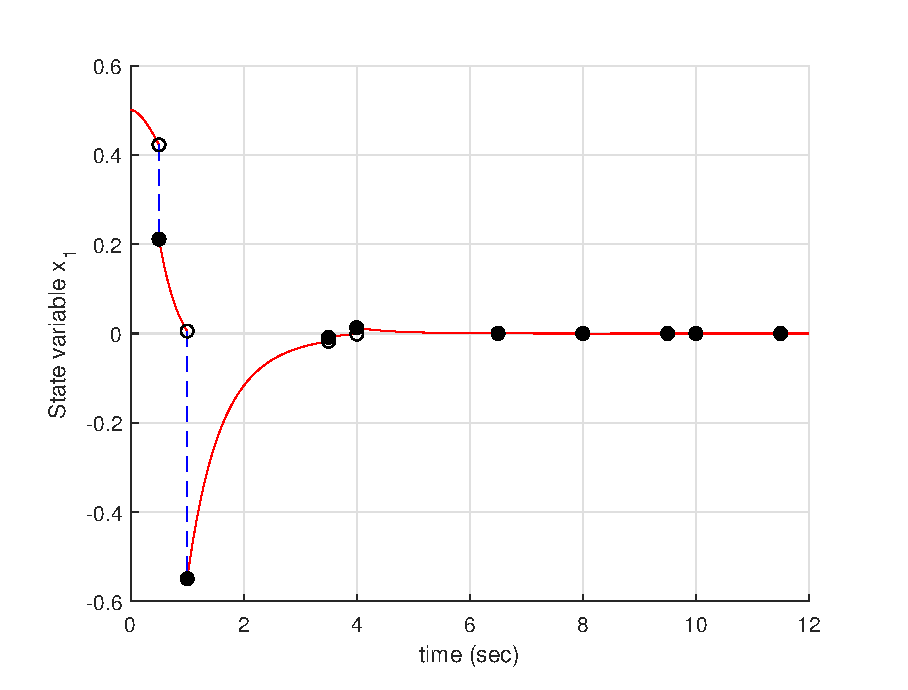
\includegraphics[scale=0.8]{FG5.eps} 
\caption{Initial Value Response $x_1(t)$ vs $t$}
\end{figure}

\begin{figure}
\centering
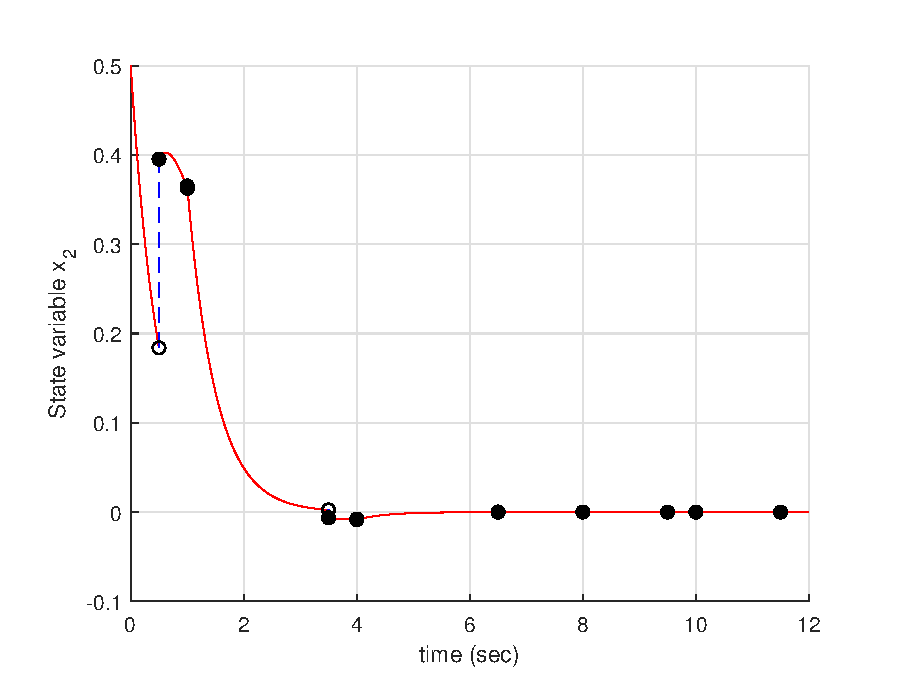
\includegraphics[scale=0.8]{FG6.eps} 
\caption{Initial Value Response $x_2(t)$ vs $t$}
\end{figure}

\begin{figure}
\centering
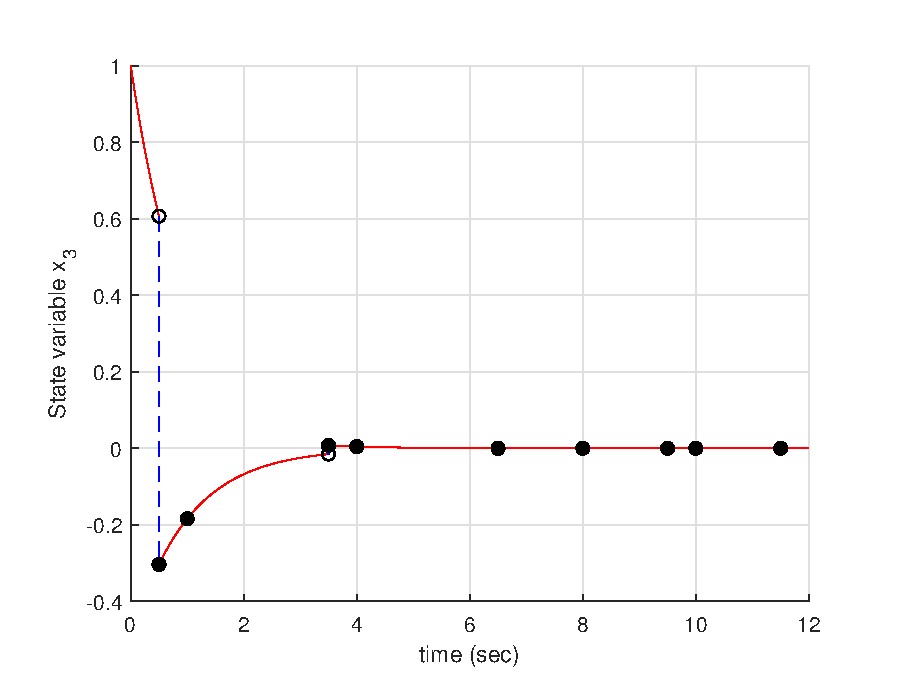
\includegraphics[scale=0.8]{FG7.eps} 
\caption{Initial Value Response $x_3(t)$ vs $t$}
\end{figure}

\begin{figure}
\centering
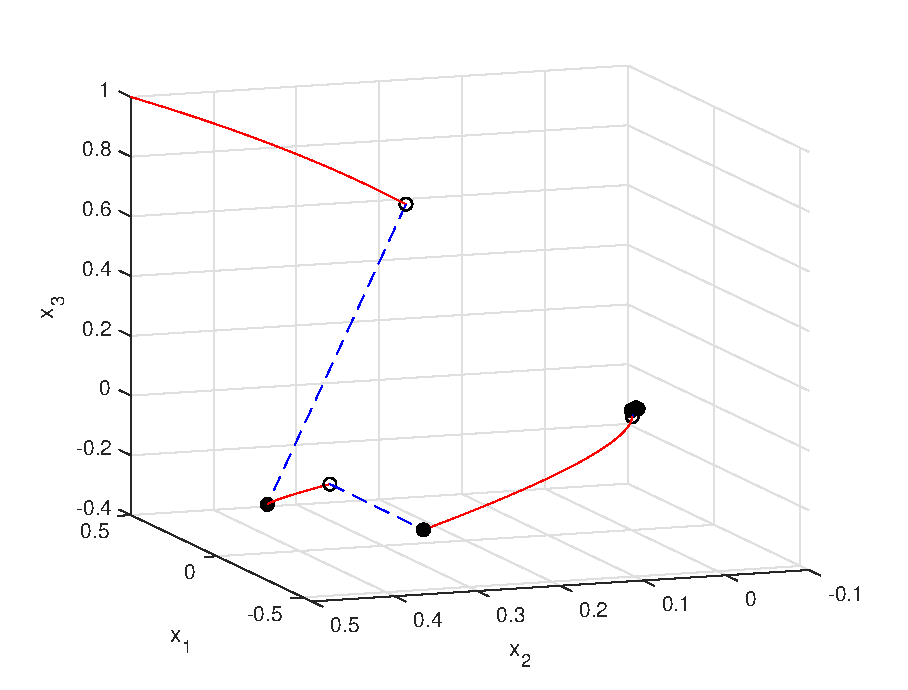
\includegraphics[scale=0.8]{FG8.eps} 
\caption{Phase Portrait}
\end{figure}

\begin{figure}
\centering
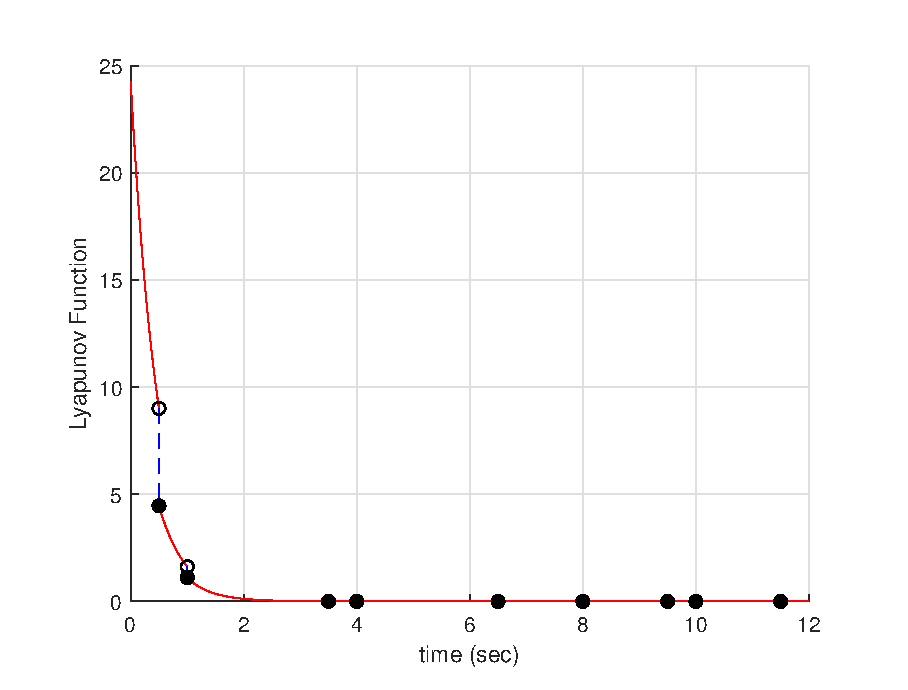
\includegraphics[scale=0.8]{FG9.eps} 
\caption{Lyapunov Function $V[x(t)]$ vs $t$}
\end{figure}

\pagebreak

\begin{theorem} ([1, Theorem 4.5]) Let $\mathsf{L} = \mathsf{Rad} ( \mathsf{L} ) \oplus \mathsf{S}$ denote a Levi decomposition of the impulsive Lie algebra.  If the Levi factor $\mathsf{S}$ is compact, then the linear impulsive system (1) is UES.
\end{theorem}

\textbf{Example 15.} In this example we also consider a 3-dimensional linear impulsive system in the form of (1) with data matrices $\mathrm{A}_\mathcal{C}$ and $\mathrm{A}_\mathcal{I}$ given by
$$
A_{\mathcal{C}} = 
	\left[
	\begin{aligned}
	-1/4 && -1/4 &&  0  \\
	   2 && -1/4 && -2  \\
	   0 &&  1/4 && -1/4
	\end{aligned}
	\right]\,,
\qquad		
A_{\mathcal{I}} = 
	\left[
	\begin{aligned}
	 1/4 && -1/2  && 1/4 \\
	 1/4 &&    0  && -1/4  \\
	 1/4 &&  1/2  && 1/4
	\end{aligned}
	\right]\,
$$

Similar to Example 14, we follow the Algorithms in Section 3 to compute the impulsive Lie algebra and its radical and Levi factor. We also create simulation for the system with respect to a set of impulse times and then plot the state trajectories and 3-dimensional state portrait. In the case that the Levi factor is not compact, we make a conclusion of the UES according to the behavior of the state trajectories and state portrait of the system. \\

First, applying Algorithm 2 produces the four-dimensional impulsive Lie algebra $\mathsf{L}$ with a basis given by
$$
\mathfrak{B} = \{ 
	\left[
	\begin{aligned}
	 1 && 0 &&  0  \\
	 0 && 1 &&  0  \\
	 0 && 0 &&  1
	\end{aligned}
	\right]\,,
\text{ }		
	\left[
	\begin{aligned}
	 0 && 0 && 0 \\
	 1 && 0 && -1  \\
	 0 && 0 && 0
	\end{aligned}
	\right]\,,
\text{ }		
	\left[
	\begin{aligned}
	 0 && 0 && 1 \\
	 0 && 3 && 0  \\
	 1 && 0 && 0
	\end{aligned}
	\right]\,,
	\text{ }		
	\left[
	\begin{aligned}
	 0 && 1 && 0 \\
	 0 && 0 && 0  \\
	 0 && -1 && 0
	\end{aligned}
	\right]\,
	\}
$$

Next, by applying Algorithm 3 we obtain the one-dimensional radical with a basis below
$$
\mathfrak{B}_\mathsf{R} = \{ 
	\left[
	\begin{aligned}
	 1 && 0 &&  0  \\
	 0 && 1 &&  0  \\
	 0 && 0 &&  1
	\end{aligned}
	\right]\,
	\}
$$

Direct calculation shows $[\mathfrak{B},\mathfrak{B}_{\mathsf{R}}] = 0$ or $[\mathsf{L},\mathsf{Rad}(\mathsf{L})] = 0$. Hence, the radical is also the center of $\mathsf{L}$, and so the Lie algebra is reductive. Next, implementing Algorithm 4 gives us a Levi factor $\mathsf{S}$ of $\mathsf{L}$, generated by
$$ \mathfrak{B}_{\mathsf{S}} =
\{
	\left[
	\begin{aligned}
	 0 && 0 && 0 \\
	 1 && 0 && -1  \\
	 0 && 0 && 0
	\end{aligned}
	\right]\,, \text{ }
	\left[
	   \begin{aligned}
		 -1 && 0 && 1  \\
	 	 0 &&  2 && 0  \\
	 	 1 &&  0 && -1
	   \end{aligned}
	  \right]\,, \text{ }
\left[
	\begin{aligned}
	 0 && 1 && 0 \\
	 0 && 0 && 0  \\
	 0 && -1 && 0
	\end{aligned}
	\right]\,
\}
$$ 

If the Killing form of the Levi factor is not negative definite, then the Levi factor is not compact. Running the MATLAB function for computing Killing form (see Appendix A) produces a matrix of the Killing form of the Levi factor as
$$
[\mathcal{K}_{\mathsf{S}}] = 
	\left[
	\begin{aligned}
	 0 &&  0 &&  8  \\
	 0 && 32 &&  0  \\
	 8 &&  0 &&  0
	\end{aligned}
	\right]\,
$$

It is clear that $[\mathcal{K}_{\mathsf{S}}]$ is not negative definite (as the 1-by-1 leading principal minor is zero, and eigenvalues of $[\mathcal{K}_{\mathsf{S}}]$ are -8, 8, 32). Hence, $\mathcal{K}_{\mathsf{S}}$ is not negative definite. This implies, from Definition 25, that the Levi factor $\mathsf{S}$ is not compact.\\

Since the Levi factor is not compact, we have no conclusion (based on Theorem 6) of whether or not the system is UES. However, the result can be drawn from the behavior of the state trajectories and the state portrait of the system. The system is stimulated and plotted with respect to the initial state and the set of impulse times as given below respectively
$$
x_0 = 
\begin{bmatrix}
1 \\
0 \\
-1
\end{bmatrix},
$$
$$
\mathcal{T} = \{k \frac{\pi}{2} , \text{ } k = 1,...,10 \}
$$

From the graphs (Figure 10-13), the behavior of the state trajectories graphically indicates that the system is not uniformly exponentially stable. \\ 
\\
\\
\\
\\
\\
\\

\begin{figure}
\centering
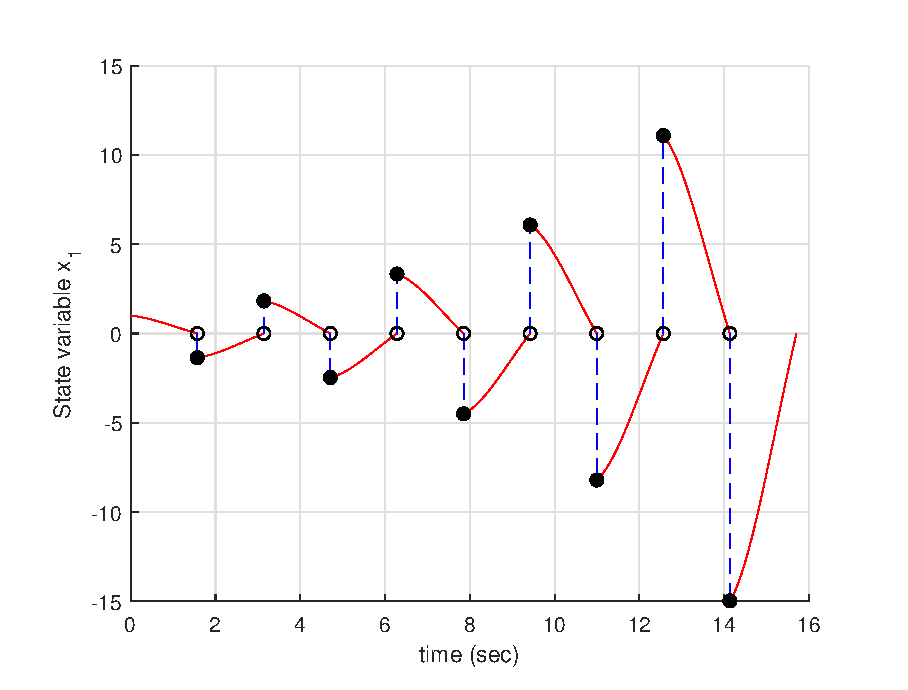
\includegraphics[scale=0.8]{FG10.eps} 
\caption{Initial Value Response $x_1(t)$ vs $t$}
\end{figure}

\begin{figure}
\centering
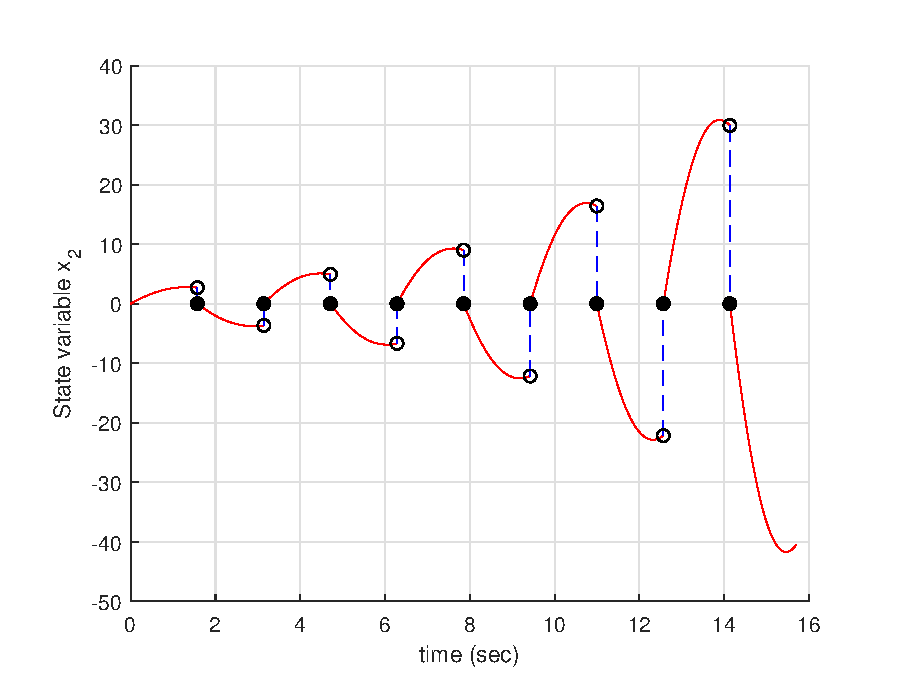
\includegraphics[scale=0.8]{FG11.eps} 
\caption{Initial Value Response $x_2(t)$ vs $t$}
\end{figure}

\begin{figure}
\centering
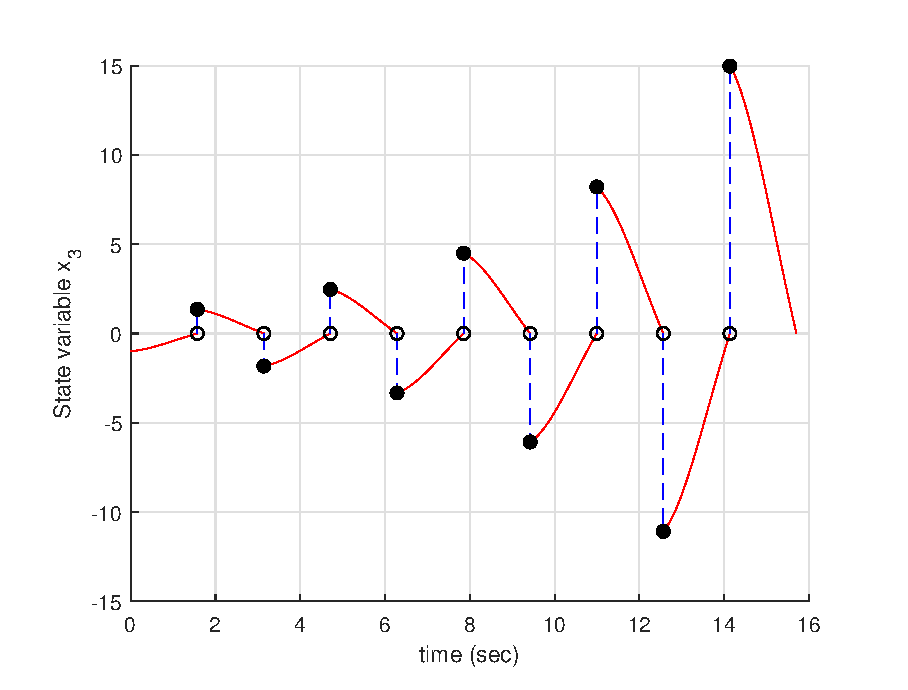
\includegraphics[scale=0.7]{FG12.eps} 
\caption{Initial Value Response $x_3(t)$ vs $t$}
\end{figure}

\begin{figure}
\centering
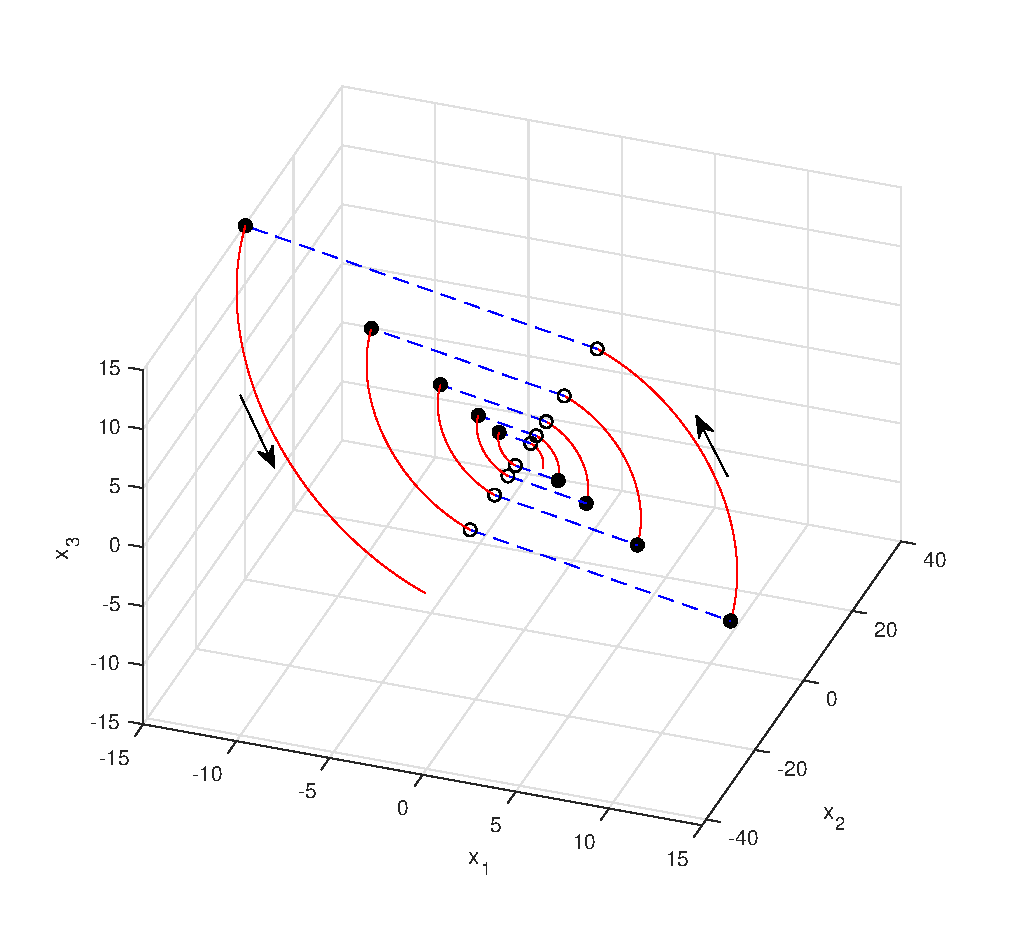
\includegraphics[scale=0.7]{FG13.eps} 
\caption{Phase Portrait}
\end{figure}

%
\pagebreak
\section{Conclusion}
\qquad This research project has investigated uniform exponential stability for linear impulsive systems using Lie algebraic techniques in which we have focused on the computation of the Levi decomposition of the impulsive Lie algebra. The goal of the project is mainly intended to develop computational tools for executing the Levi decomposition using MATLAB. Our primary contribution is the development of convenient computational tools which can provide tutorial values and thus effectively support academic ideas and uses. For this purpose, the computational tools have been developed in the particular manner that all algorithms must preserve "nice" numbers-integers or rational numbers and better illustrate the underlying theory and algorithms presented in the project. The traditional MATLAB commands do not meet these aims and objectives. We have designed computational tools that satisfy the goal. In particular, our accomplishments involve the following:

\begin{enumerate}
\item Algorithm and MATLAB implementation for a complement to a subspace in a given subspace and solving matrix equations that preserve nice numbers (integers and rationals),

\item Algorithm and MATLAB implementation for the minimal invariant subspace containing a specified subspace

\item Algorithm and MATLAB implementation for the impulsive Lie algebra,

\item Algorithm and MATLAB implementation for the derived Lie algebra of any Lie algebra,

\item Algorithm and MATLAB implementation for structure constants for any Lie algebra,

\item Algorithm and MATLAB implementation for Killing form of any Lie algebra,

\item Algorithm and MATLAB implementation for the radical of any Lie algebra,

\item Algorithm and MATLAB implementation for a Levi factor of the Lie algebra in the reductive case.
\end{enumerate}

However, the computational tools for the case that the radical is not the center have not been completed. This suggests topics for further work. Specifically, our future research would concentrate on the two more general cases. The first case is that the radical is Abelian but not equal to the center and the second is that the radical is not required to be Abelian. 


\pagebreak
\begin{thebibliography}{}

\bibitem{Lawrence 1}
D. A. Lawrence.
Lie-algebraic stability conditions for stability of linear impulsive systems.
In \textit{Proceedings of the 2013 American Control Conference}, pages 3185-3190, 2013.

\bibitem{Lawrence 2}
D. A. Lawrence.
On the uniform exponential stability of linear impulsive systems.
In \textit{Proceedings of the 2017 American Control Conference}, pages 1250-1256, 2017.

\bibitem{Lawrence 3}
N. Nguyen and D. A. Lawrence.
On the Lie algebra of a linear impulsive systems.
In \textit{Proceedings of the 2018 American Control Conference}, pages 430-435, 2018.
 
\bibitem{Liberzon 1} 
D. Liberzon, J. P. Hespanha, and S. Morse.
Stability of switched systems: a Lie-algebraic condition. 
\textit{Systems} \& \textit{Control Letters}, 37:117-122, 1996.

\bibitem{Agrachev 1} 
A. A. Agrachev and D. Liberzon.
Lie-algebraic stability criteria for switched systems. 
\textit{SIAM Journal on Control and Optimization}, 40(1):253-269, 2001.

\bibitem{Yang 2}
T. Yang.
\textit{Impulsive Systems and Control: Theory and Applications}.
Nova Science Publishers, 2001.

\bibitem{Dagli} 
M. Dagli.
\textit{Levi Decomposition of Lie Algebras; Algorithm for its Computation}.
MS. thesis, Iowa State University, Department of Mathematics, 2004.

\bibitem{Zassenhaus 1}
H. Zassenhaus.
\textit{Lie Groups, Lie Algebras and Representation Theory}.
Presses University Montreal, 1981.

\bibitem{Erdmann}
K. Erdmann and M. J Wildon.
\textit{Introduction to Lie Algebras}.
Springer-Verlag, London, 2006.

\bibitem{de Graaf}
W. A. de Graaf.
\textit{Lie Algebras Theory and Algorithms}.
Elsevier Science, 2000.

\bibitem{Graham}
A. Graham. 
\textit{Kronecker Products and Matrix Calculus with Applications}.
Ellis Horwood Limited, Chichester, 1981.

\bibitem{Steeb 1}
W.-H Steeb. 
\textit{Problems and Solutions in Introductory and Advanced Matrix Calculus}.
World Scientific, 2006.

\bibitem{Meyer}
C. D. Meyer.
\textit{Matrix Analysis and Applied Linear Algebra}. 
SIAM, 2000.

\end{thebibliography}

\pagebreak

\begin{appendices}
\section{MATLAB CODE}

\begin{verbatim}

% COMPUTING THE MINIMAL INVARIANT SUBSPACES

function M = min_inv(T,B)
% T is a linear transformation (matrix), B is a matrix
% Initialization

M1 = B;
[R, jb] = rref(M1);
r1 = length(jb); % r1 = rank(M1);
condition = 1;
while condition
   r0 = r1;
   M  = M1;
   M1 = [B T*M];
   [R1, jb1] = rref(M1);
   r1 = length(jb1); % r1 = rank(M1);
   condition = (r1 > r0);
end
[R2, jb2] = rref(M');
r2 = length(jb2);
M = R2(1:r2,:)';
\end{verbatim}

\begin{verbatim}
	
% COMPUTING IMPULSIVE LIE ALGEBRA

function L = Lie(A,g)
ad_A = ad_A_of(A);
Ad_g_inv = Ad_g_inv_of(g);

L_0 = min_inv(Ad_g_inv, vec(A));
L_1 = add(L_0, min_inv(Ad_g_inv, ad_A*L_0));

N1 = L_0;
[R, jb] = rref(N1);
r1 = length(jb); % r1 = rank(N1);
condition = 1;

while condition
   r0 = r1;
   N  = N1;
   N1 = add(L_0, min_inv(Ad_g_inv, ad_A*N));
   [R1, jb1] = rref(N1);
   r1 = length(jb1); 
   condition = (r1 > r0);
end

[R2,jb2] = rref(N');
r2 = length(jb2);
L = R2(1:r2,:)'; % In matrix form
\end{verbatim}

\begin{verbatim}

%COMPUTING THE DERIVED ALGEBRA

function L_pr  = der_al(L)
% L is a matrix whose columns constitute a basis for L
k = 1;
[R,jb] = rref(L);
d = length(jb);  %d = rank(L);

if d == 1
    L_pr = []; % L is Abelian
else
    for i=1:d-1
        for j=i+1:d
        B = bracket(vec_inv(L(:,i)),vec_inv(L(:,j)));
        STORAGE(:,k) = vec(B);
        k = k+1;
        end
    end
[R1,jb1] = rref(STORAGE');
r = length(jb1);   % r = rank(STORAGE);
    if r == 0
        L_pr = []; % L is Abelian
    else
        L_pr = R1(1:r,:)';
    end
end
\end{verbatim}

\begin{verbatim}

% COMPUTING STRUCTURE CONSTANTS

function ad_X = str_cons(L,L1)
k = 1;
[r1,d1] = size(L);  % d1 = the dimension of L;
[r2,d2] = size(L1); % d2 = the dimension of L1
% Calculating structure constants
for j=1:d2
    for i=1:d1
        Z = bracket(vec_inv(L1(:,j)),vec_inv(L(:,i)));
        STORAGE(:,k) = coor(L,Z);
        k = k+1;
    end
end

% Calculating adjoint representation of L1
[row,c] = size(STORAGE);
r = 1;
m = 1;
n = d1;
while n <= c
    C(:,:,r) = STORAGE(:,m:n);
    r = r+1;
    m = n+1;
    n = r*d1;
end
ad_X = C; % Return a three dimensional array

\end{verbatim}

\begin{verbatim}

% COMPUTING THE KILLING FORM

function Kill = Kill_form(L,L1)
ad_X = str_cons(L,L);
ad_Y = str_cons(L,L1);

[r,c] = size(L); % c is the dimension of L
[r1,c1] = size(L1); % c1 is the dimension of L1

% Finding Killing form with respect to L and L_pr
for j=1:c1
    for i=1:c
        K(j,i) = trace(ad_X(:,:,i)*ad_Y(:,:,j));
    end
end
Kill = K; % Return a matrix
\end{verbatim}

\begin{verbatim}

% COMPUTING THE RADICAL OF A LIE ALGEBRA L

function Radical = rad(L)
L1 = der_al(L); % The derived algebra of L
[r,c] = size(L); 
[r1,c1] = size(L1);
if c1 == 0
    Radical = L;  % L is solvable
elseif c1 == c
    Radical = []; % L is semisimple
else
Kill = Kill_form(L,L1); % The Killing form

% Calculating coefficients alpha
alpha = null(Kill,'r');
    % if norm(alpha) == 0; or if alpha = zeros(size(alpha))
    %    Radical = [];
    % else
    
% A set of basis vectors for the radical is linear combinations
% of basis vectors X_i in L and alpha
[r_alpha,c_alpha] = size(alpha);
for n = 1:c_alpha
    b = 0; % b is a c-by-1 vector
        for k = 1:c
        b = b + alpha(k,n)*L(:,k);
        end;
    STORAGE(:,n) = b;
    % Rad(:,:,n) = vec_inv(b);
end;

Radical = STORAGE;  % Return a matrix 
end
\end{verbatim}

\begin{verbatim}

% COMPUTING A LEVI FACTOR 

function Levi_factor = Levi(L)
R = rad(L);
[r,c] = size(L);
[r1,c1] = size(R);
if c1 == c
    Levi_factor = []; % L is solvable
elseif c1 == 0
    Levi_factor = L;  % L is semisimple
else

% The complement of R in L is
Com = comp(L,R);
L1 = [Com R];
% Find structure constants for the quotient space L/R
% L/R <--> {x1_bar, x2_bar ... xm_bar} ~ C <--> {x1, x2 ... xm}
ad_X = str_cons(L1,L1); % Recalculate a set of structure constants for L
                        % with respect to a new basis [C R]
[r,c,p] = size(ad_X);
   for k = 1:p-1
       B = ad_X(:,:,k);
       [r_b,c_b] = size(B);
       % ad_X_bar are induced map from ad_X
       ad_X_bar(:,:,k) = B(1:r_b-1,1:c_b-1); % Delete last columns and last rows
                                             % of ad_Xk
   end
   
   % STEP 1 (RIGHT-HAND SIDE): Calculating the right-hand side tube b_ij of 
   % the EQUATION
   % and STEP 3 (LEFT-HAND SIDE): Calculating the Matrix in the left-hand side of 
   % the EQUATION
   [r1,c1,p1] = size(ad_X_bar);
   column = 1;
   for k = 1:p1-1                      % k is the index of page
       for j = k+1:p1                  % j is the index of column
           Xk = vec_inv(Com(:,k));
           Xj = vec_inv(Com(:,j));
           tube(:,column) = vec(bracket(Xk,Xj)) - Com*ad_X_bar(:,j,k);
           % RIGHT-HAND SIDE
           % There are p1(p1-1)/2 = m(m-1)/2
           b = ad_X_bar(:,j,k);
           Matrix_trans(:,column) = b; % LEFT-HAND SIDE
           column = column+1;
       end
   end

% STEP 2(LEFT-HAND SIDE): Calculating the Yij (scalars) in the left-hand side
% of the EQUATION
   Yij_trans = mat_sol(R,tube); % Yij is a column vector
   Yij = Yij_trans';

   Matrix = Matrix_trans';

   alpha = mat_sol(Matrix,Yij); % alpha is a matrix in which column i goes
                             % with r_i

   % STEP 4: Computing a basis for a Levi factor using the following
   % transformations yi = xi + sum(apha_ji*r_j), i = 1...m
   [r_alpha,c_alpha] = size(alpha);
   for i = 1:r_alpha
       yi = Com(:,i) + R*alpha(i,:)';
       Levi_factor(:,i) = yi; 
    end
end

\end{verbatim}

\begin{verbatim}

% SIMULATION

function [simulation, time] = simimp(A,g,Delta,t0,x0)
% A and g are data matrices
% Tau is a set of impulse times given in a row vector
% t0 is an nitial time
% x0 is an initial state

sysA  = ss(A, [], eye(size(A)), []);

d = length(Delta);
Tau(1) = t0;
for j = 2:d+1
    T = Tau(j-1) + Delta(j-1);
    Tau(j) = T;
end
Tau;

time  = [];
impulse_state = [];

xp   = x0;

l    = length(Tau);

for k = 1:l-1
    tt = 0:0.01:Delta(k);
    xx = initial(sysA, xp, tt)';
    impulse_state = [impulse_state xx];
    time = [time tt+Tau(k)];
    xn = xx(:, end);
    xp = g * xn;
end

simulation = impulse_state;
\end{verbatim}

\begin{verbatim}

% SOLVING MATRIX EQUATION AX = B

function [X_particular, S_0, matrix_solver] = mat_sol(A,B)
% A is a matrix and B is a matrix
[R,jb] = rref(A);
r_0 = length(jb);
  
A_aug = [A B];
[R1,jb] = rref(A_aug);
r_aug = length(jb);

if r_0 == r_aug
% We just solve the system when it is consistent, i.e. r = r_aug
% Determine the pivot variables and the particular solution
    [r,c] = size(A);
    [r1,c1] = size(B);
    X_p = zeros(c,1); % initialize
    
    k=1;
    for i = 1:c1
        X_p(jb) = R1(1:r_aug,c+i);
        X_par(:,k) = X_p;
        k = k+1;
    end
    X_particular = X_par;
    % Determine the parameterized set of the associated
    % homogeneous equation
    S_0 = null(A,'r');

    % Determine the general solution for the nonhomogeneous equation
    matrix_solver = [X_par S_0];
    
else disp('The equation is not consistent');
    [X_particular, S_0, matrix_solver] = [];
end

\end{verbatim}
\end{appendices}


\end{document}

































